% Abstract for this chapter
%
%**********************************************************************
In this chapter,
we discuss motion tasks suitable for execution under reactionless motion control,
with a seven-DoF redundant manipulator.
First, we will show that the reactionless motion of the model consists of the predominant wrist and elbow motion.
Based on these motions,
we propose the following three tasks \cite{Sone2015}:
(i) inspection task using a hand-held camera,
(ii) point-to-point position control,
(iii) deployment task from a stowed configuration.
The performance of these tasks are verified via numerical simulation.

%%%%%%%%%%%%%%%%%%%%%%%%%%%%%%%%
\section{Manipulator model}
\label{sec:MODEL}
%%%%%%%%%%%%%%%%%%%%%%%%%%%%%%%%
%%%%%%%%%%%%%%%%%%%%%%%%%%%%%%%%
\subsection{Model description}
%%%%%%%%%%%%%%%%%%%%%%%%%%%%%%%%

%
% ---------------------------------------------------------------------
\begin{figure}[t]
  \centering
  \begin{minipage}{0.25\linewidth}
    \centering
    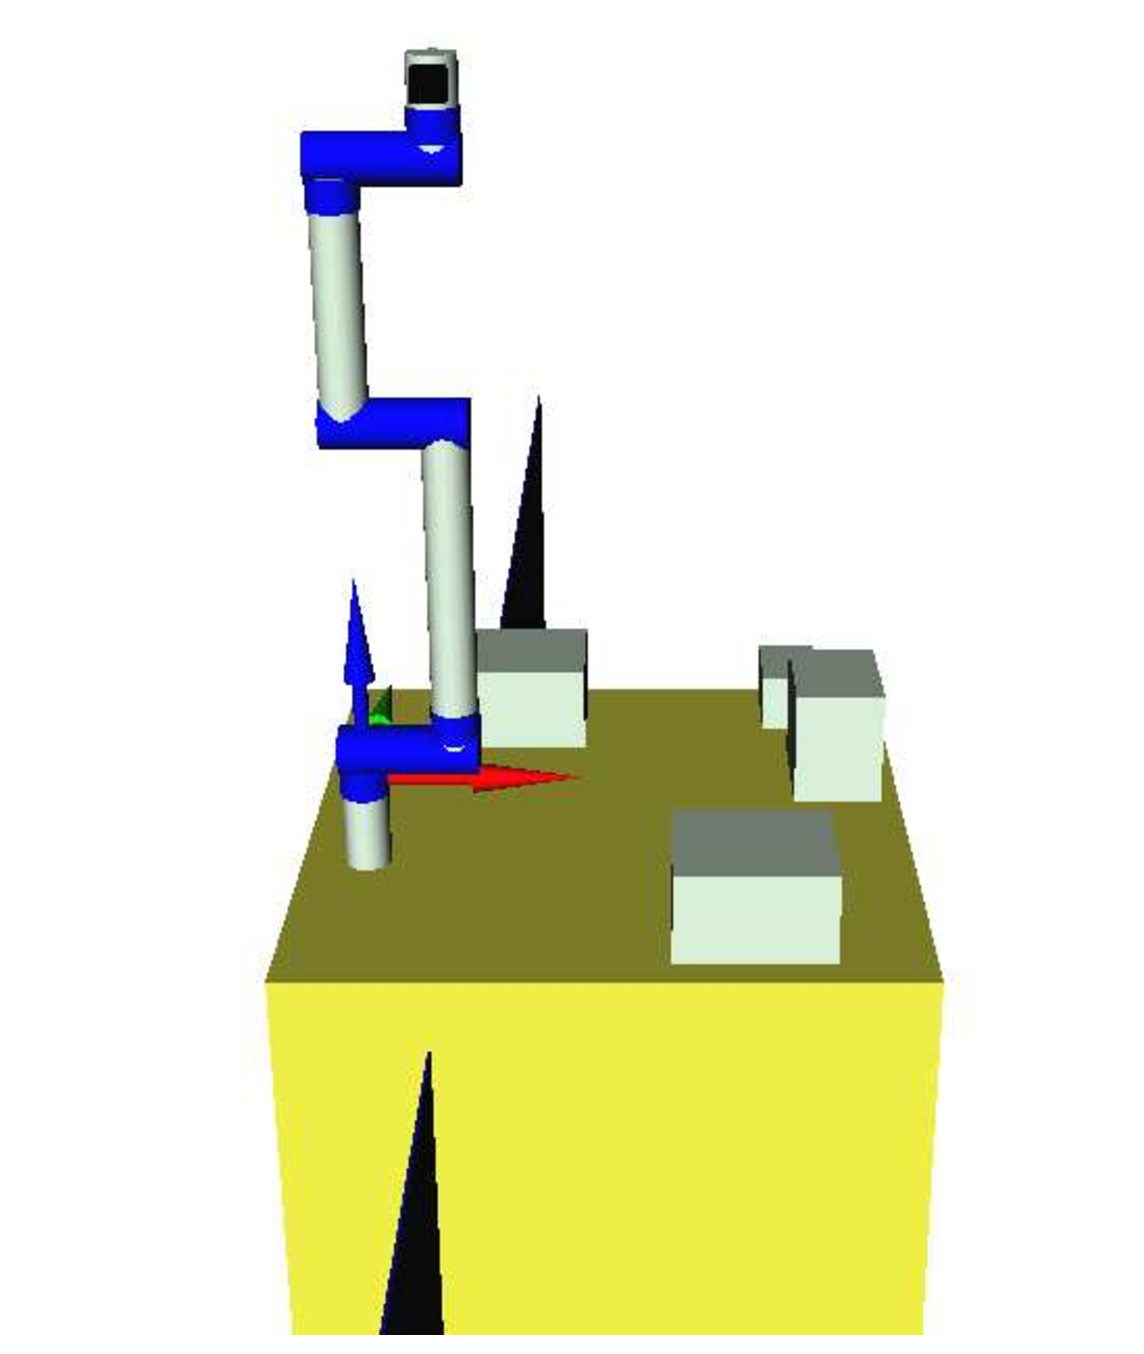
\includegraphics[width=1.0\linewidth]{fig/chapter4/init.eps}
  \end{minipage}
  \begin{minipage}{0.65\linewidth}
    \centering
    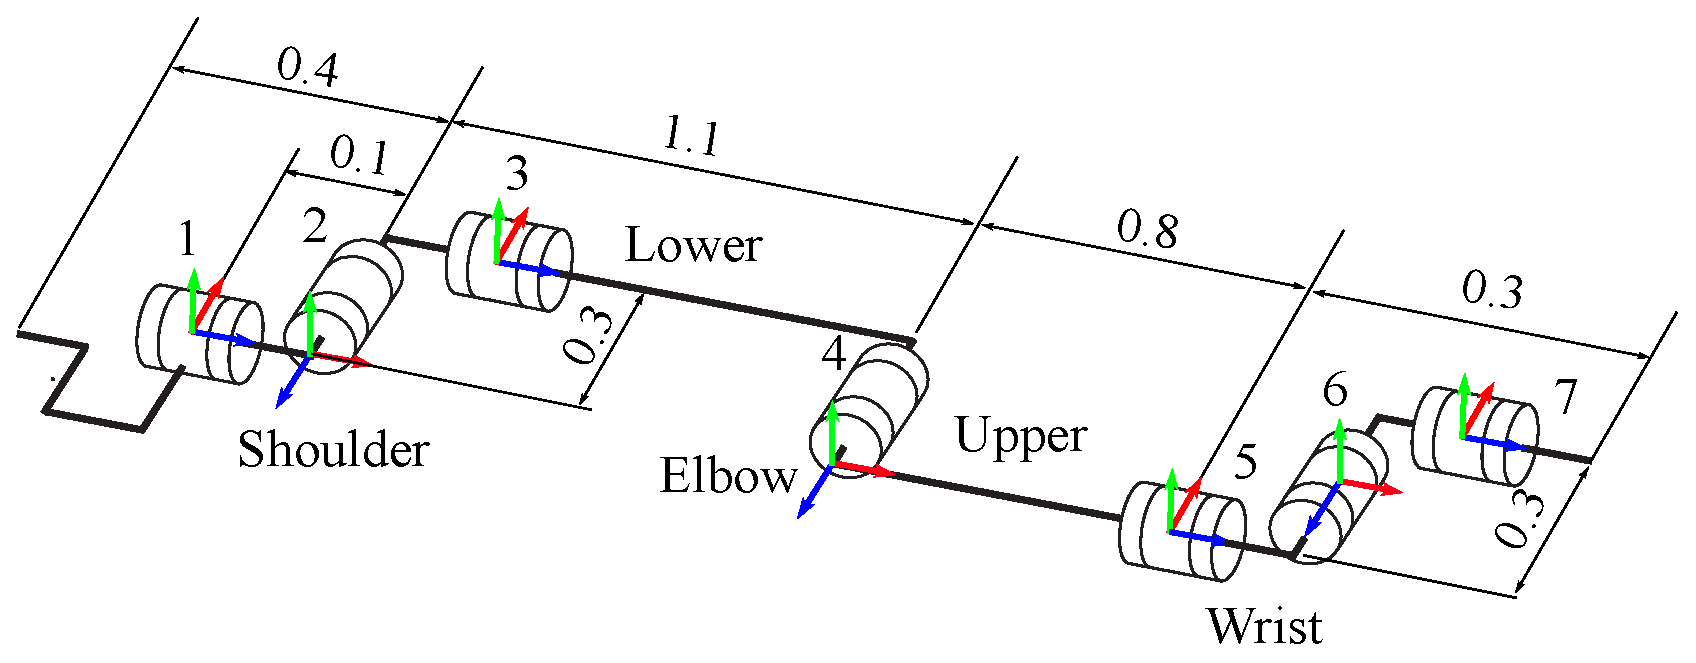
\includegraphics[width=1.0\linewidth]{fig/chapter4/typeA_7R.eps}    
  \end{minipage}
  \caption{Our manipulator model with seven-DoF mechanism at the initial configuration ($\theta_{i} = 0\unit{rad},~\forall\theta_{i}$).}
  \label{fig:MODEL}
\end{figure}
% ---------------------------------------------------------------------
%
We consider a free-flying space robot model consisting of a satellite base,
and a serial-link seven-DoF kinematically redundant manipulator.
The manipulator is characterized by a kinematic chain with a distinctive lower/upper arm
subchain, including a rotational ``elbow'' joint, a ``shoulder'' and a ``wrist'' joint, all of them  
with offsets. The kinematic structure and simulation model are displayed in \fig{MODEL}.
The manipulator attachment position is determined from the ETS-VII design, at $[-0.79~-0.29~1.0]^{T}\unit{m}$
with respect to the base CoM coordinate frame \cite{Yoshida2003}.
The dynamic model parameters are shown in \tab{parameter}.
%
% ---------------------------------------------------------------------
\begin{table}[t]
  \centering
  \caption{Dynamic model parameters}
  \begin{tabular}[h]{c||c|c|c|c}\hline\hline
    & Mass [kg]&
    \multicolumn{3}{ c }{Inertia moment [$\mathrm{kgm^{2}}$]}\\\hline
    $i$ & $m_{i}$&  $I_{xi}$ & $I_{yi}$ & $I_{zi}$ \\\hline\hline
    1 & 30.0 & 0.0671 & 0.0671& 0.0851\\\hline
    2 & 30.0 & 0.0843& 0.267 & 0.267\\\hline
    3 & 45.0 & 3.81 & 3.81& 0.127 \\\hline
    4 & 40.0 & 0.113& 2.19 & 2.19\\\hline
    5 & 20.0 & 0.213 & 0.213 & 0.0250\\\hline
    6 & 20.0 & 0.0250 & 0.0292 & 0.0292\\\hline
    7 & 25.0 & 0.0990& 0.0990 & 0.0313\\\hline
  \end{tabular}
  \label{tab:parameter}
\end{table}
% ---------------------------------------------------------------------
%
%%%%%%%%%%%%%%%%%%%%%%%%%%%%%%%%%%%%%%%%%%%%%%%%%%
\subsection{Reactionless motion representation}
%%%%%%%%%%%%%%%%%%%%%%%%%%%%%%%%%%%%%%%%%%%%%%%%%%

Before proceeding with the analysis of the reactionless motion task,
we have to identify the reactionless motion capability with the manipulator model.
First, note that the DoF of reactionless motion is four, 
which is obtained as the difference between the number of joints (seven) 
and the base attitude variables (three).
The following discussion provides a useful representation of the four-DoF reactionless motion.

For the analysis, we divide the kinematic chain into two subchains: 
the positioning subchain comprising  joints 1 through 4, and the wrist subchain 
comprising the rest of the joints. Then, we focus on the amplitude of the angular momentum 
produced by each of the two subchains. Because of the serial-link structure, the  wrist subchain is 
characterized with relatively small mass and length of the moment arm. 

Dividing joint velocity into the positioning and wrist subchain related terms,
we can rewrite the reactionless constraint as follows:
%
% ---------------------------------------------------------------------
\begin{align}
  \tbm{M}_{P\omega m}\thd_{P} + \tbm{M}_{W\omega m}\thd_{W} = \bm{0}
\end{align}
% ---------------------------------------------------------------------
%
where $\thd = [\thd_{P}~\thd_{W}]$,
$\tbm{M}_{\omega m} = [\tbm{M}_{P\omega m}~\tbm{M}_{W\omega m}]$;
$(\circ)_{P}$ and $(\circ)_{W}$ represent the quantities related to the positioning and wrist subchains.
In the above equation, the first term is the partial angular momentum produced by the positioning subchain;
the second term is stemming from the wrist subchain.

Next, we focus on the amplitude of these angular momentum.
Because of the small mass and the length of moment arm of the wrist subchain,
the angular momentum produced by the motion of the wrist subchain will be far smaller than that
obtained from the positioning subchain. Therefore, we can assume that the positioning subchain 
can compensate the base disturbance induced by the wrist subchain motion, completely.
This implies one particular reactionless motion patterns, characterized with ``unconstrained'' 
wrist motion plus small compensating variations in the positioning subchain, as shown in \fig{motion}~(a).
This motion is a three-DoF reactionless motion and is referred to  as
the {\sl predominant wrist motion}, hereafter.
This motion can be obtained as follows:
%
% ---------------------------------------------------------------------
\begin{align}
  \thd = \bmat{\bm{B}(\th) \\ \bm{E}}\thd_{W}\label{eq:RL_POS}
\end{align}
% ---------------------------------------------------------------------
%
where $\bm{B} = -\tbm{M}_{P\omega m}^{+}\tbm{M}_{W\omega m}\R{4 \times 3}$
is a linear map from the wrist subchain motion to the
positioning subchain motion ensuring the reactionless constraint.

%
% ---------------------------------------------------------------------
\begin{figure}[t]
  \centering
  \begin{minipage}[h]{0.4\linewidth}
    \centering
    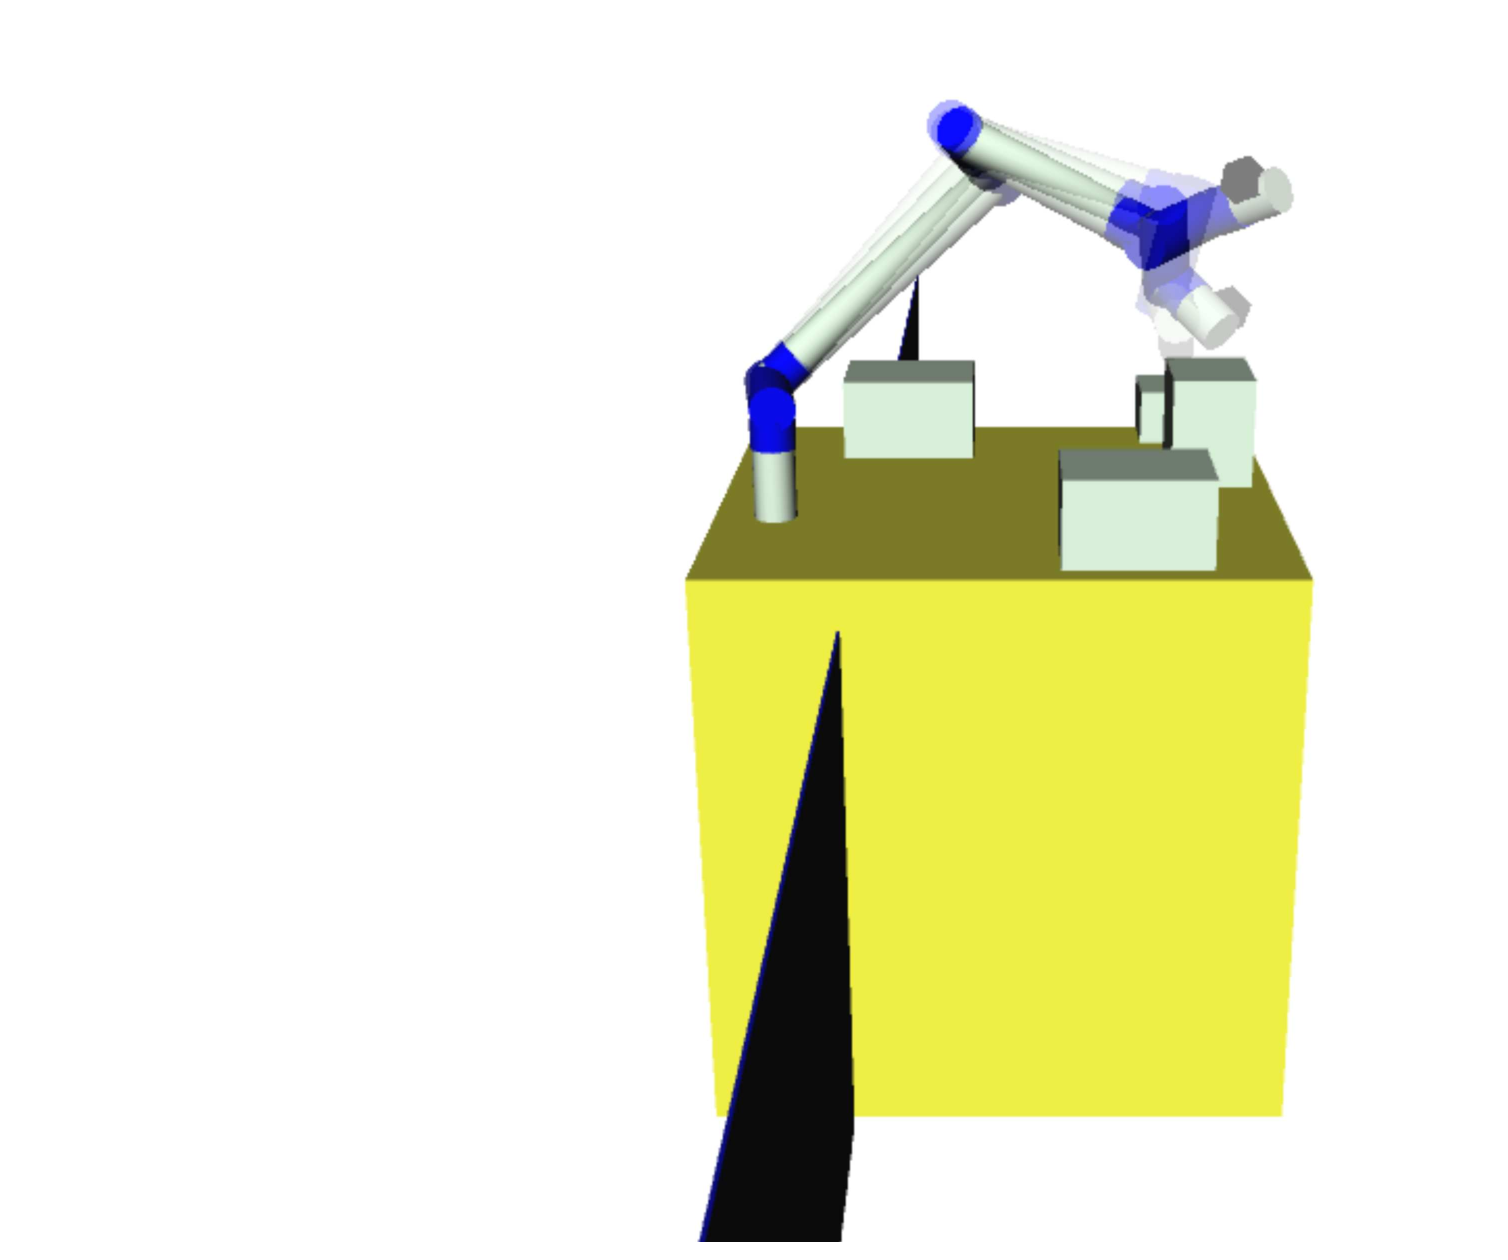
\includegraphics[width=1.0\linewidth]{fig/chapter4/spatial/WS.eps}
    \footnotesize\par{(a)}
  \end{minipage}
  \begin{minipage}[h]{0.4\linewidth}
    \centering
    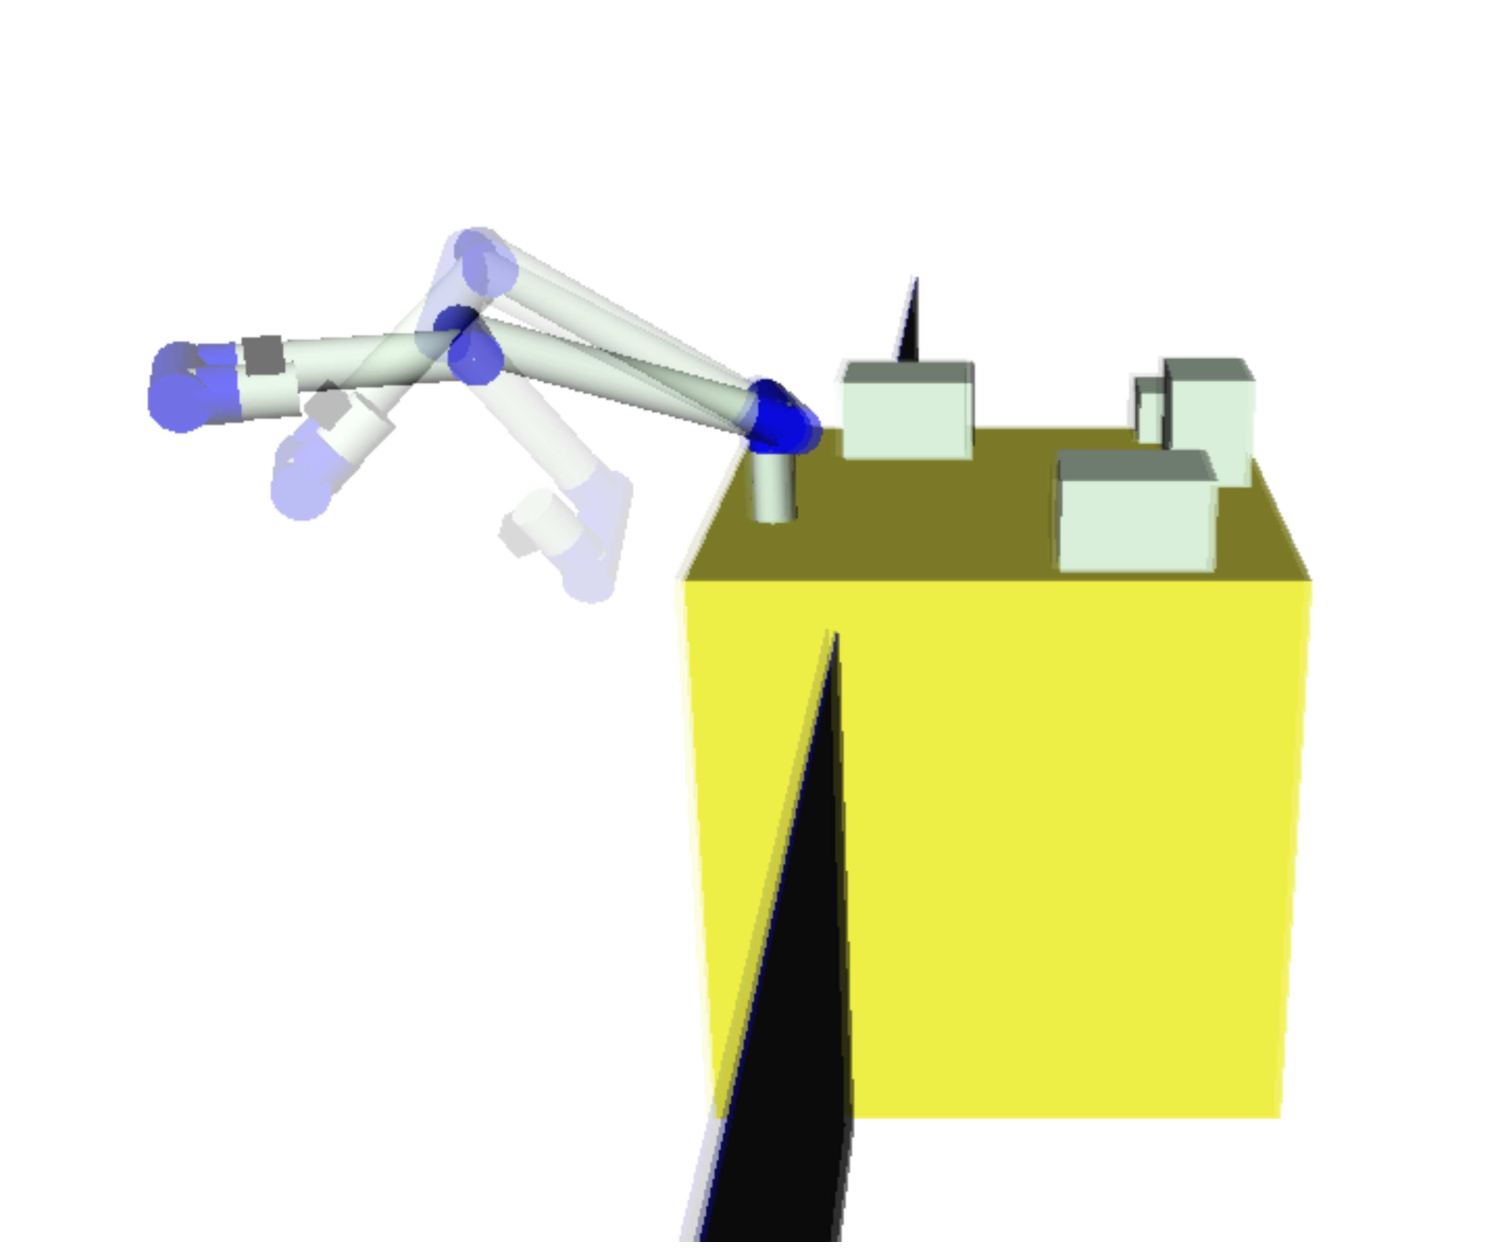
\includegraphics[width=1.0\linewidth]{fig/chapter4/spatial/PS.eps}
    \footnotesize\par{(b)}
  \end{minipage}
  \caption{Reactionless motion of the manipulator model: (a) the predominant wrist motion and (b) the elbow folding motion.}
  \label{fig:motion}
\end{figure}
% ---------------------------------------------------------------------
%

The remaining one-DoF reactionless motion is uniquely determined from the null-space vector
of the coupling inertia submatrix that is related to the positioning subchain $\tilde{\bm{M}}_{\omega mP}$.
%
% ---------------------------------------------------------------------
\begin{align}
  \thd = b \bmat{\bm{n}(\th) \\ \bm{0}}
\end{align}
% ---------------------------------------------------------------------
%
where $b$ is an arbitrary scalar.
From the angular momentum conservation, we can assume that motions in Joints 1 and 2 will be
relatively small for  the above two reactionless motion patterns.
Hence, this motion approximately consists of the elbow folding/unfolding motion as shown in \fig{motion}~(b).

Since these two patterns are  orthogonal, their superposition will represent all possible reactionless
motions for the given manipulator model, as follows:
%
% ---------------------------------------------------------------------
\begin{align}
  \thd &= \bmat{\bm{B}(\th) \\ \bm{E}}\thd_{W} + b \bmat{\bm{n}(\th) \\ \bm{0}}
\end{align}
% ---------------------------------------------------------------------
%
From the above analysis,
we can then arrive at the following conclusion:
because the end-effector position largely depends on the motion in the positioning subchain,
it follows that under reactionless motion, the positioning DoF of end-effector will be 
approximately one. This feature results only from the specific kinematic structure of the
positioning subchain, comprising two upper/lower arm links (i.e.\ it is similar to the 
two-link planar example discussed previously).
Therefore, we will henceforth focus on reactionless end-effector orientation control
with the predominant wrist motion and reactionless manipulator configuration control.
This makes our research different from previous studies.

Based on the two type of reactionless motions,
we propose the following three tasks for reactionless motion:
(i) inspection task using a hand-held camera,
(ii) point-to-point positioning task and
(iii) deployment task from a stowed configuration.
First, we describe the inspection task in what follows.

%%%%%%%%%%%%%%%%%%%%%%%%%%%%%%%%%%%%%%%%%%%%%%%%%%%%%%%%%%%
\section{Inspection task using a hand-held camera}
\label{sec:INSPECTION}
%%%%%%%%%%%%%%%%%%%%%%%%%%%%%%%%%%%%%%%%%%%%%%%%%%%%%%%%%%%

%
% ---------------------------------------------------------------------
\begin{figure}[t]
  \centering
  \begin{minipage}[h]{0.495\linewidth}
    \centering
    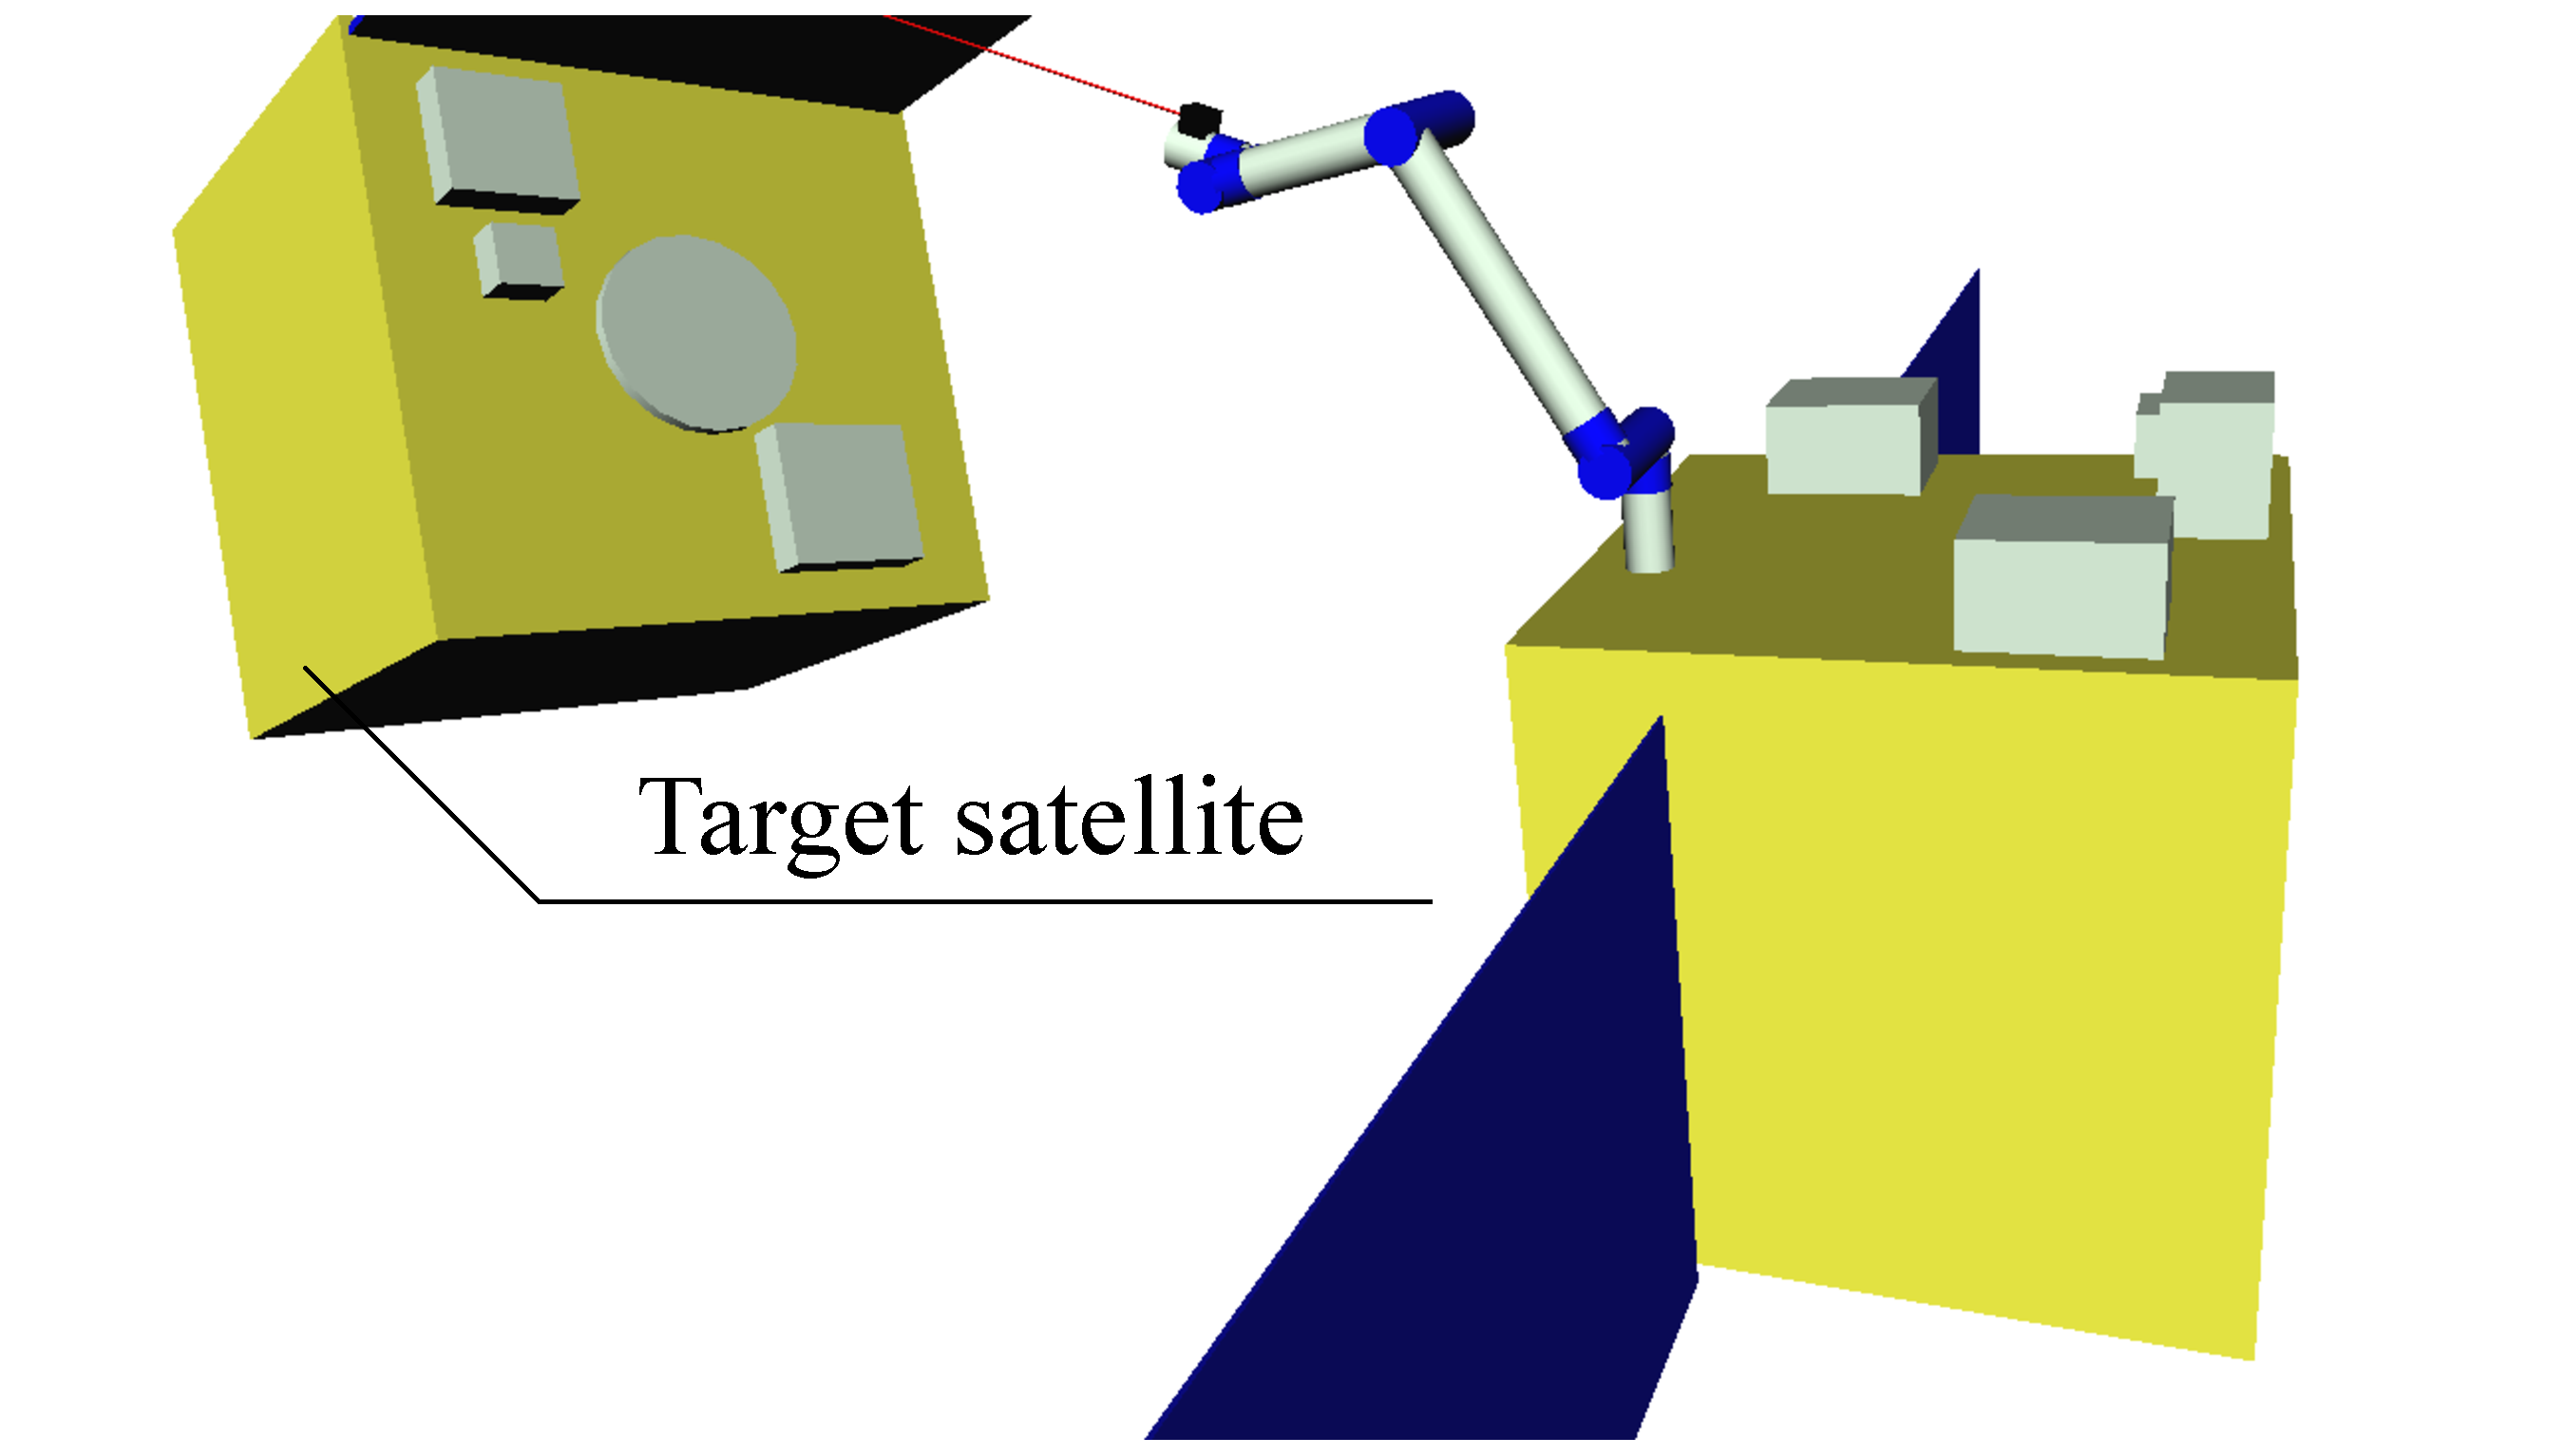
\includegraphics[width=1.0\linewidth]{fig/chapter4/inspection/observation.eps}
    \footnotesize\par{(a)}
  \end{minipage}
  \begin{minipage}[h]{0.495\linewidth}
    \centering
    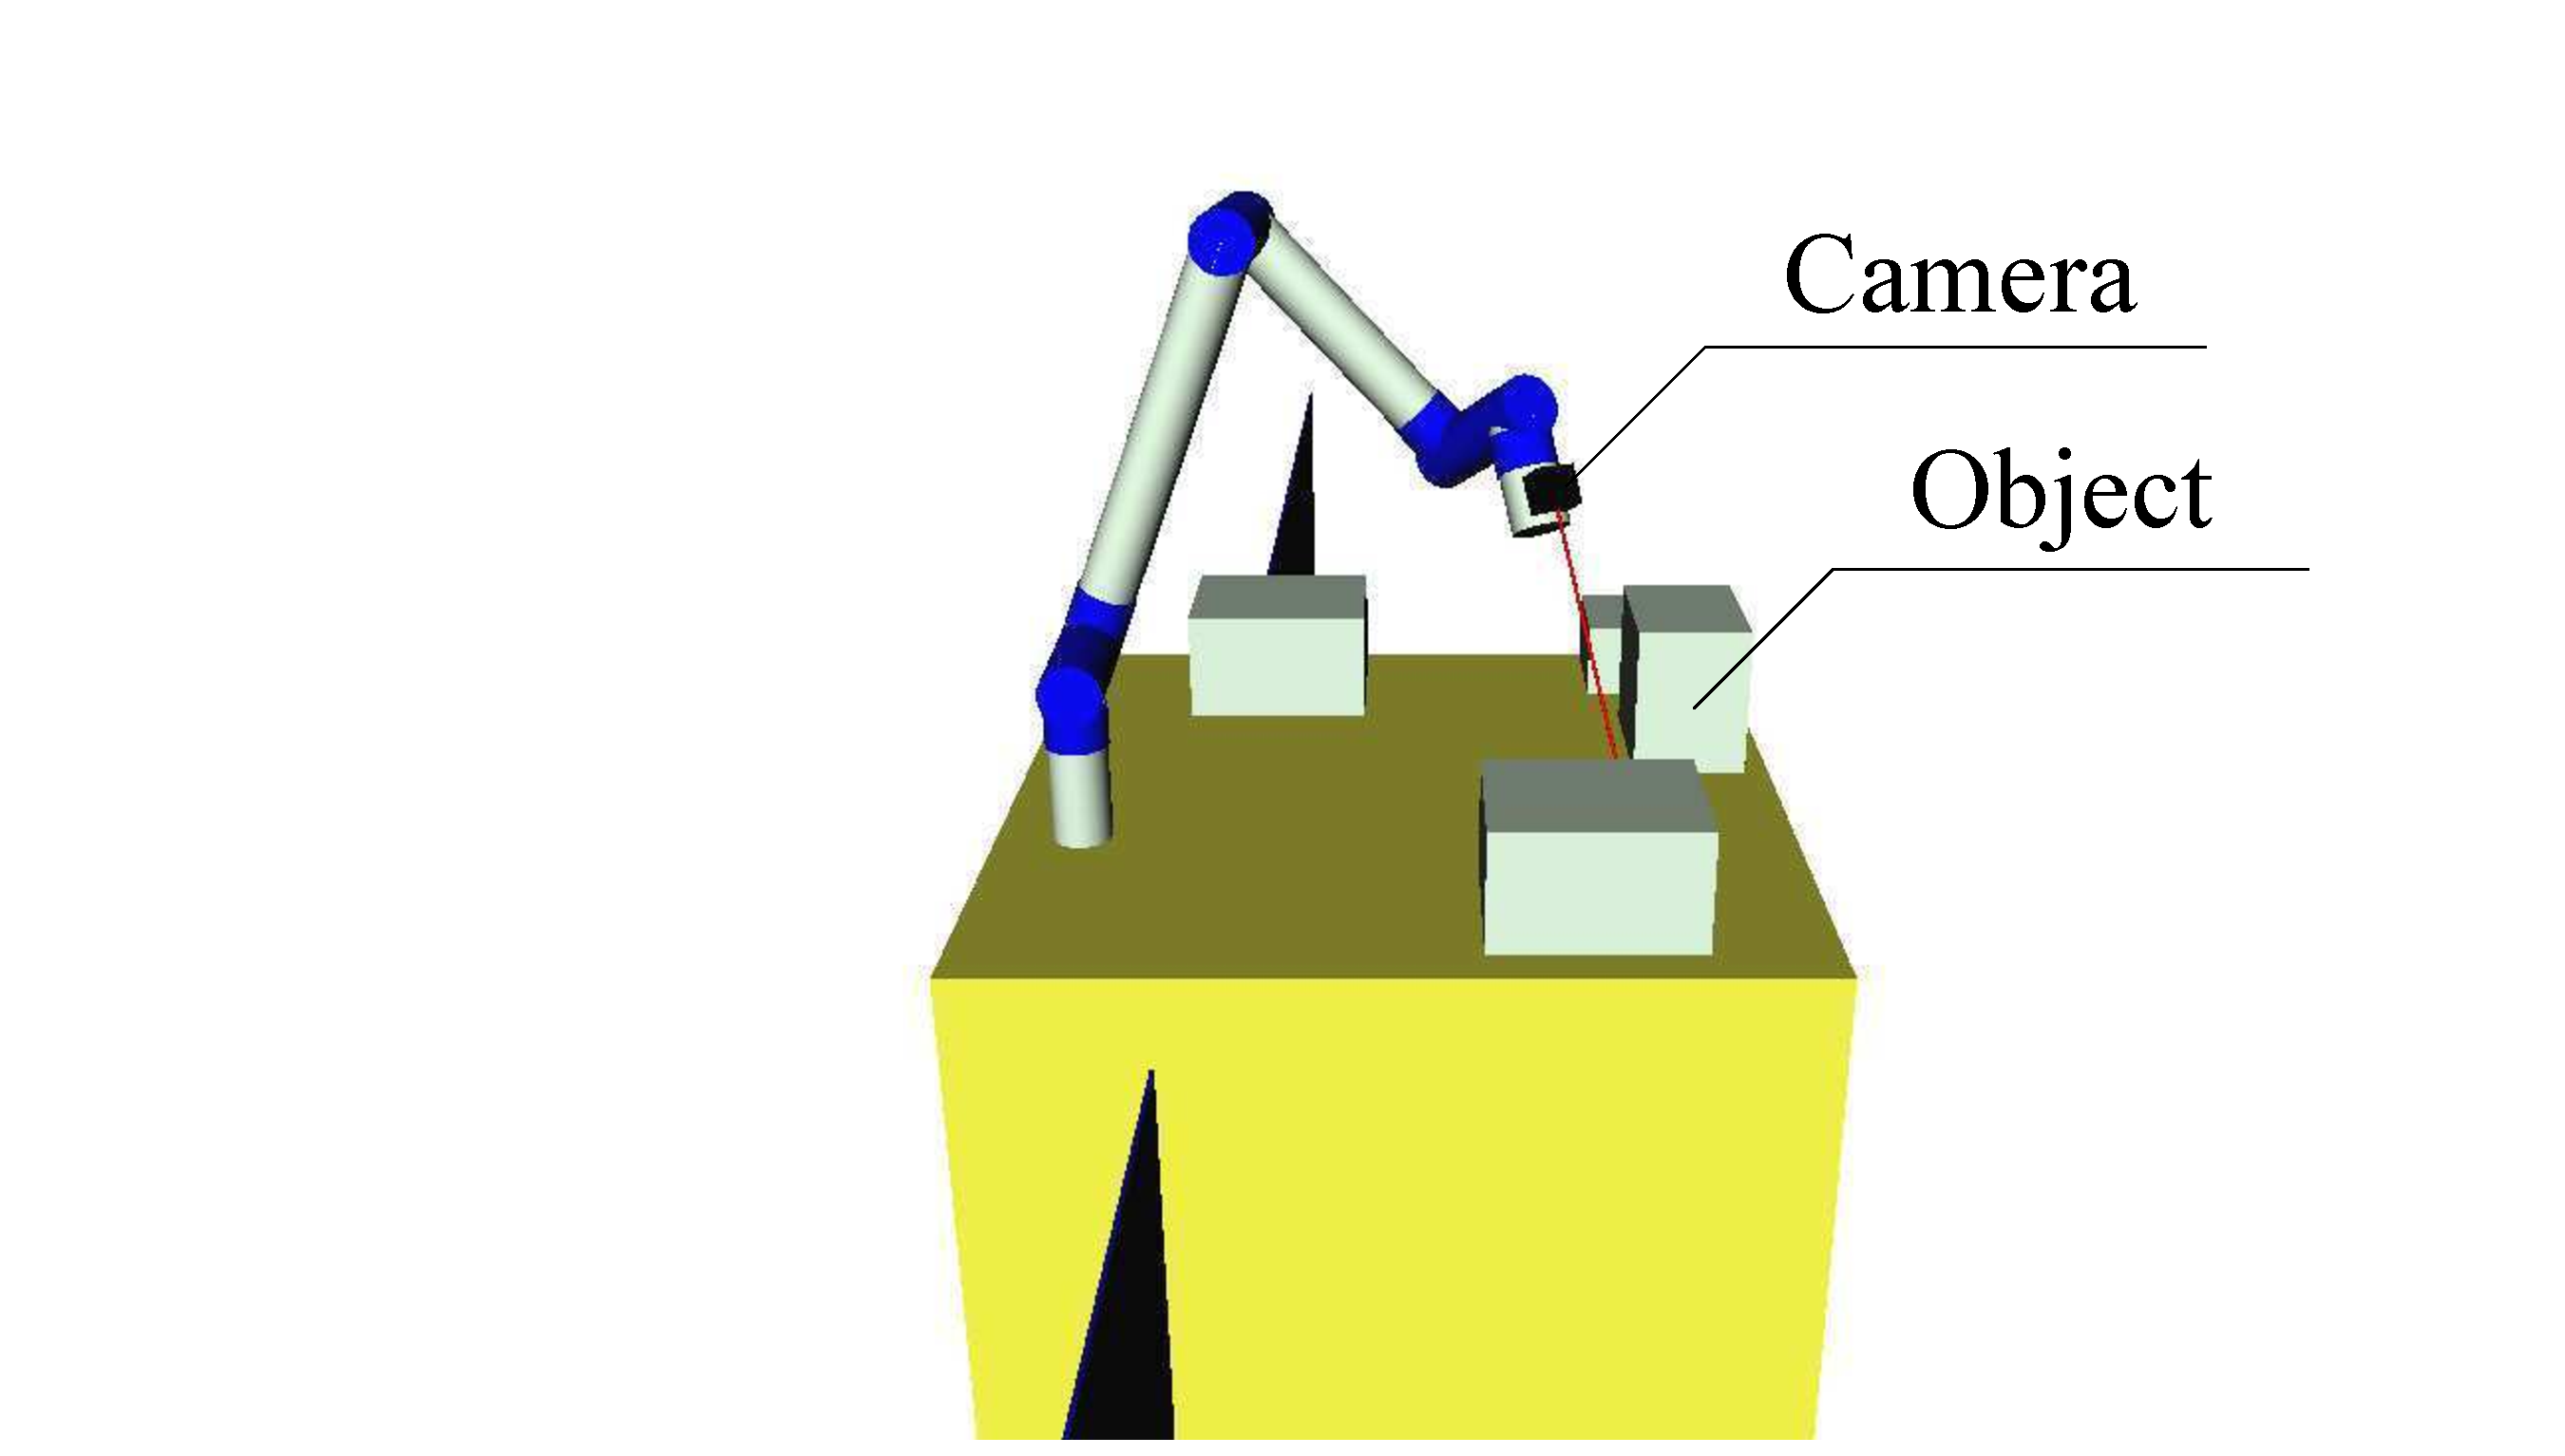
\includegraphics[width=1.0\linewidth]{fig/chapter4/inspection/inspection.eps}
    \footnotesize\par{(b)}
  \end{minipage}
  \caption{Inspection task using the hand-held camera: 
    (a) target satellite to be refueled of captured and (b) own-satellite attached devices.}
  \label{fig:ins}
\end{figure}
% ---------------------------------------------------------------------
%
One frequently appearing task for free-floating space robots is inspection with a hand-held camera 
of devices mounted on the own satellite base or on the satellite to be serviced, 
as shown in \fig{ins}.
Such task was also performed within the ETS-VII mission \cite{Oda1997} but without using 
reactionless control. For camera inspection, once the arm is positioned appropriately,
the camera view angle for inspection is changed by rotating the wrist.
This task is  expected to be performed multiple times during a number of missions,
such as construction, maintenance, debris removal and so on.
Hence, this task is a good candidate for execution under reactionless motion control
for improved work efficiency.

The following three control subtasks are considered necessary to accomplish  camera inspection.
%
% ---------------------------------------------------------------------
\begin{enumerate}
\item Reactionless constraint of the base attitude (three-DoF).
\item Orientation control of the wrist (three-DoF).
\item Stabilization of the wrist position.
\end{enumerate}
% ---------------------------------------------------------------------
%
The first control subtask ensures reactionless motion. The second one is essential for camera 
inspection. The third control subtask is necessary to avoid a large deflection of the wrist from the 
initial position, since there is no position control subtask.
The above subtasks will be simultaneously realized through  consecutive null-space projections 
\cite{Konstantinov1981, Nakamura1981}, known also as the task-of-priority approach \cite{Nakamura1987}.
Priorities are assigned among the tasks according to their relative importance.
A higher-priority task can then be accomplished without being disturbed  from the lower-priority tasks.
This is ensured by projecting lower-priority tasks onto the common null-space of 
all higher-priority tasks.


%%%%%%%%%%%%%%%%%%%%%%%%%%%%%%%%%%
\subsection{Control command}
\label{sec:CONTROLLER}
%%%%%%%%%%%%%%%%%%%%%%%%%%%%%%%%%%
The priorities are assigned as follows.  The reactionless constraint is the highest-priority subtask,
wrist orientation control is the second-priority one and wrist position stabilization is the 
lowest-priority subtask. The control command for the joint velocity  
can then be obtained as follows:
%
% ---------------------------------------------------------------------
\begin{align}
  \thd^{ref} = \bar{\bm{J}}_{\omega_{e}}^{+}\bm{\omega}_{e}^{ref} + k_{g}\bm{P}\bm{J}_{v_{w}}^{T}\Delta\bm{p}_{w}
  \label{eq:REF}
\end{align}
% ---------------------------------------------------------------------
%
where $\bm{\omega}_{e}\R{3}$ is the angular velocity of the end-effector and
$\Delta\bm{p}_{w} (= \bm{p}_{w} - \bm{p}_{w}^{init})\R{3}$ is the wrist deflection from the initial position.
Matrix $\bar{\bm{J}}_{\omega_{e}} = [\bm{J}_{\omega_{e}}\bm{P}_{RNS}]\R{3 \times 7}$ is the restricted Jacobian 
matrix \cite{Nenchev1992} for the wrist subtask. Matrices $\bm{J}_{\omega_{e}}$, $\bm{J}_{v_{w}}\R{3 \times 7}$ 
stand for the Jacobians w.r.t.\ the angular/linear velocity of the 
end-effector, respectively. 
$\bm{P} = \bm{P}_{RNS}(\bm{E} - \bar{\bm{J}}_{\omega_{e}}^{+}\bar{\bm{J}}_{\omega_{e}})$ is the combined null-space 
projector for the lowest-priority task.
$k_{g}$ is a positive gradient gain.

The structure of the control command is as follows.
The first term is the end-effector orientation control projected onto the null-space of
the coupling inertia matrix:
this term can accomplish the end-effector orientation control under the reactionless constraint.
The second term minimizes the following potential function to stabilize the wrist position:
%
% ---------------------------------------------------------------------
\begin{align}
 V = \frac{1}{2}\|\Delta\bm{p}_{w}\|^{2}.
\end{align}
% ---------------------------------------------------------------------
%
This term does not disturb the higher priority tasks because it is projected
onto the null-space of all higher priority tasks.
It should be noted that $\bar{\bm{J}}_{\omega_{e}}^{+}$ may become rank-deficient. This is an 
algorithmic singularity which occurs when the end-effector and  reactionless motion control 
subtasks  are in conflict. The details of this singularity will be described, below.

%%%%%%%%%%%%%%%%%%%%%%%%%%%%%%%%%%
\subsection{Numerical simulation}
\label{sec:SIMULATION}
%%%%%%%%%%%%%%%%%%%%%%%%%%%%%%%%%%
In what follows, we examine the performance under \eq{REF} by comparing it to
that under a conventional inverse Jacobian controller that keeps the positioning subchain motionless:
%
% ---------------------------------------------------------------------
\begin{align}
  \thd_{W}^{ref} &= \bm{J}_{W\omega_{e}}^{-1}\bm{\omega}_{e}^{ref}\\
  \thd_{P}^{ref} &= \bm{0}
\end{align}
% ---------------------------------------------------------------------
%

%
% ---------------------------------------------------------------------
\begin{figure}[t]
  \centering
  \begin{minipage}[h]{0.40\linewidth}
    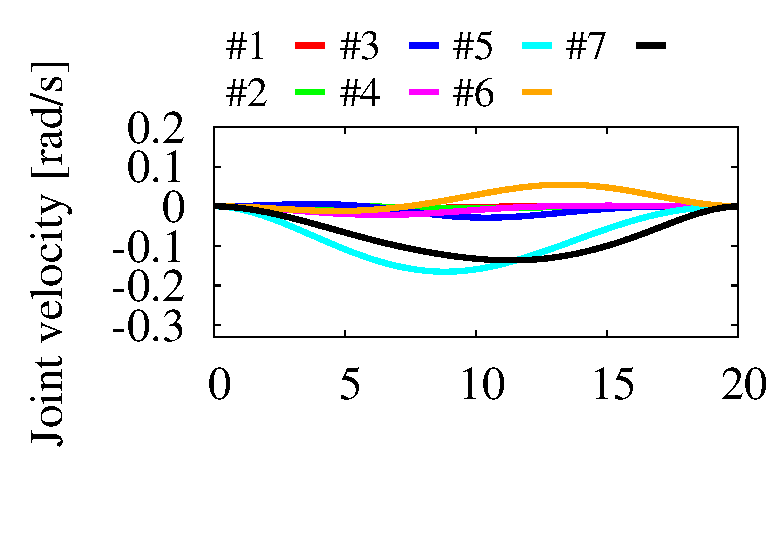
\includegraphics[width=1.0\linewidth]{fig/chapter4/inspection/case1/RL-M/U01_joint_velo.eps}
  \end{minipage}
  \begin{minipage}[h]{0.40\linewidth}
    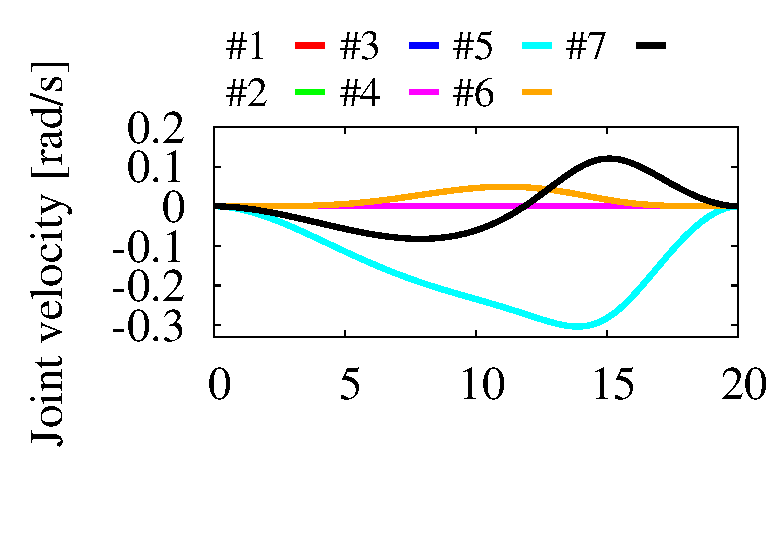
\includegraphics[width=1.0\linewidth]{fig/chapter4/inspection/case1/CONV/U01_joint_velo.eps}
  \end{minipage}\\
  \vspace{-5mm}
  \begin{minipage}[h]{0.40\linewidth}
    \includegraphics[width=1.0\linewidth]{fig/chapter4/inspection/case1/RL-M/U12_rotation_angle.eps}
  \end{minipage}
  \begin{minipage}[h]{0.40\linewidth}
    \includegraphics[width=1.0\linewidth]{fig/chapter4/inspection/case1/CONV/U12_rotation_angle.eps}
  \end{minipage}\\
  \vspace{-5mm}
  \begin{minipage}[h]{0.40\linewidth}
    \centering
    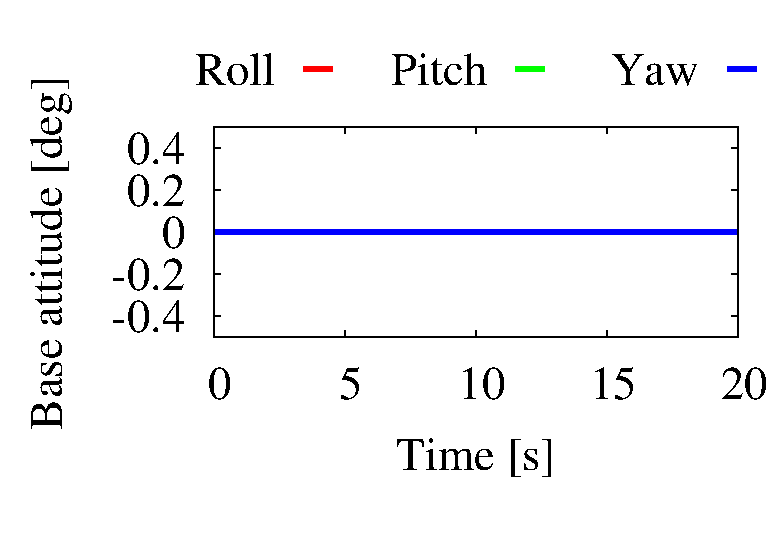
\includegraphics[width=1.0\linewidth]{fig/chapter4/inspection/case1/RL-M/X02_Base_Orientation.eps}
    \footnotesize\par{\hspace{8mm}\vspace{-2mm}Reactionless}
  \end{minipage}
  \begin{minipage}[h]{0.40\linewidth}
    \centering
    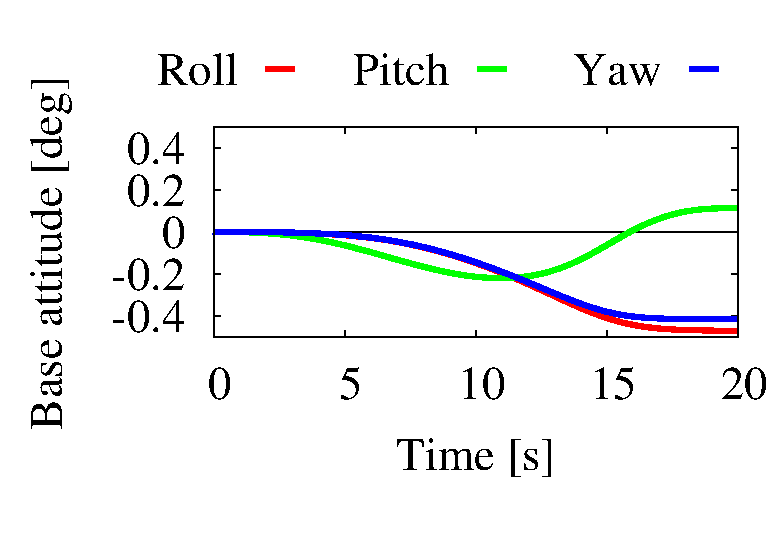
\includegraphics[width=1.0\linewidth]{fig/chapter4/inspection/case1/CONV/X02_Base_Orientation.eps}
    \footnotesize\par{\hspace{8mm}\vspace{-2mm}Conventional}
  \end{minipage}
  \vspace{1em}
  \caption{Simulation result under the satellite observation mission (\fig{ins}~(a)).}
  \label{fig:RES_INS}
\end{figure}
% ---------------------------------------------------------------------
%
We assume the following two task scenarios for observing:
(i)  a satellite to be serviced (\fig{ins}~(a)) and
(ii) the devices attached on  satellite base (\fig{ins}~(b)).
First, we verify the satellite observation case.
The initial configuration is set as $[-90~-30~0~-70~180~-30~0]^{T}\unit{deg}$ as shown in \fig{ins}~(a),
the reference angular velocity is $\bm{\omega}_{e}^{ref} = \pi[s(t)~0~0]^{T}$,
where $0 \leq s(t) \leq 1$ denotes a fifth-order spline function. 
The simulation time and the gain are set at $20\unit{s}$ and $k_{g} = 100  \unit{kg/m \cdot s}$, respectively.
The simulation results are displayed in \fig{RES_INS}.
From the angular velocity error graphs is can be seen that the end-effector task is accomplished successfully
in both simulations. Note, however, that under reactionless motion control there is no base attitude deviation.
Also, this motion is realized with a relatively small displacement of the positioning subchain, 
according to the respective joint velocity graph. In contrast, under the conventional control method
there is a relatively large base attitude deviation% 
\footnote{The maximum allowable base attitude deviation for the ETS-VII mission was about $\pm 0.05\unit{deg}$.}, 
despite the low inertia parameters of the wrist.

%
% ---------------------------------------------------------------------
\begin{figure}[t]
  \centering
  \begin{minipage}[h]{0.40\linewidth}
    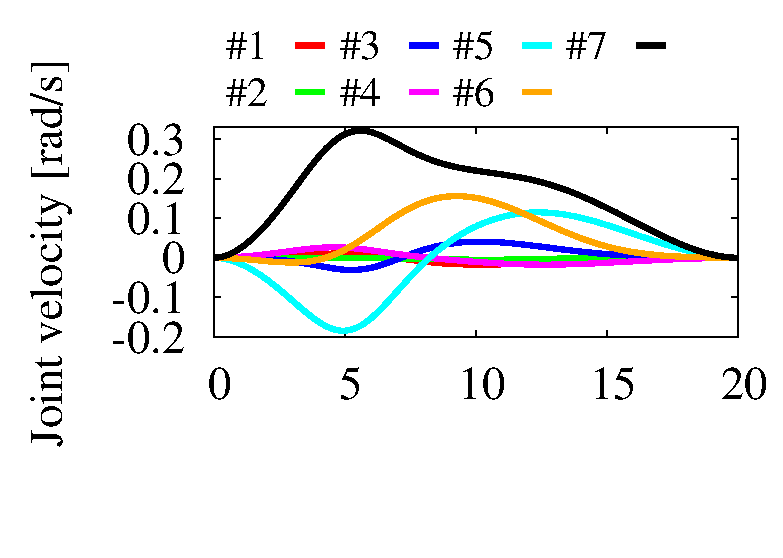
\includegraphics[width=1.0\linewidth]{fig/chapter4/inspection/case2/RL-M/U01_joint_velo.eps}
  \end{minipage}
  \begin{minipage}[h]{0.40\linewidth}
    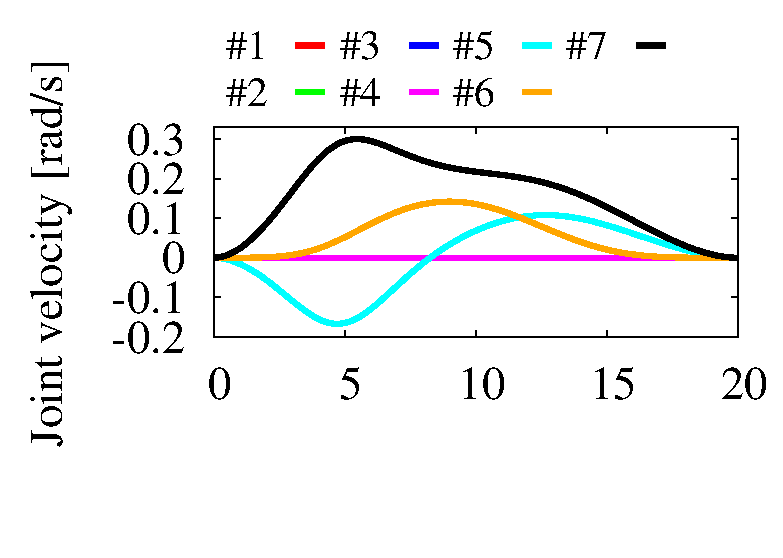
\includegraphics[width=1.0\linewidth]{fig/chapter4/inspection/case2/CONV/U01_joint_velo.eps}
  \end{minipage}\\
  \vspace{-5mm}
  \begin{minipage}[h]{0.40\linewidth}
    \centering
    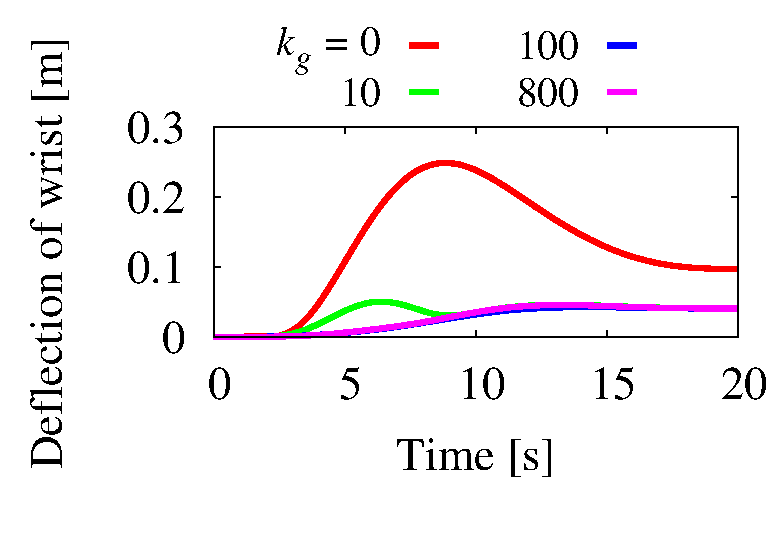
\includegraphics[width=1.0\linewidth]{fig/chapter4/inspection/case2/RL-M/U13_wrist_deflection.eps}
    \footnotesize\par{\hspace{8mm}\vspace{-2mm}Reactionless}
  \end{minipage}
  \begin{minipage}[h]{0.40\linewidth}
    \centering
    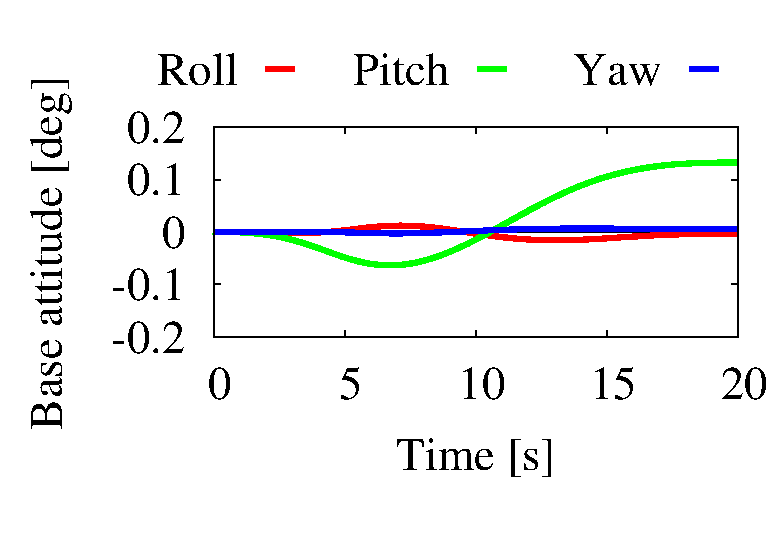
\includegraphics[width=1.0\linewidth]{fig/chapter4/inspection/case2/CONV/X02_Base_Orientation.eps}
    \footnotesize\par{\hspace{8mm}\vspace{-2mm}Conventional}
  \end{minipage}
  \vspace{1em}
  \caption{Simulation result under the inspection of own-satellite mounted devices (\fig{ins}~(b)).}
  \label{fig:RES_INS2}
\end{figure}
% ---------------------------------------------------------------------
%
In the second scenario, 
we assume that the initial configuration is set to $[90~-20~180~110~0~20~0]^{T}\unit{deg}$ as shown in \fig{ins}~(b),
the desired end-effector velocity is $\bm{\omega}_{e}^{ref} = \pi[0~0~-s(t)]^{T}\unit{rad/s}$.
The other conditions are the same as in the previous simulation.
The simulation results are shown in \fig{RES_INS2}.
First, it becomes apparent that also in this case, the base remains undisturbed under reactionless motion
while under conventional control,  a relatively large base attitude deviation is observed. 
Under reactionless motion, the effect of the cost function leads to a sufficiently small deviation from
the initial wrist position as shown in \fig{RES_INS2}.

In summary, a somewhat surprising result was obtained with the conventional controller:
a relatively large base attitude deviation was  observed despite the small mass and inertia moment 
of the wrist subchain. We can then conclude that reactionless camera inspection is useful  
to overcome this problem.

%%%%%%%%%%%%%%%%%%%%%%%%%%%%%%%%%%%%%%%%%%%%%%%%%%%%%%%%%
\section{Singularities within the inspection task}
\label{sec:SINGULAR}
%%%%%%%%%%%%%%%%%%%%%%%%%%%%%%%%%%%%%%%%%%%%%%%%%%%%%%%%%
%%%%%%%%%%%%%%%%%%%%%%%%%%%%%%%%%
\subsection{Problem statement}
\label{sec:PROBLEM}
%%%%%%%%%%%%%%%%%%%%%%%%%%%%%%%%%
In this section, we deal with possible singularities that could be encountered during 
the proposed reactionless task. There are three types of such singularities, as follows:
\begin{itemize}
\item Kinematic singularity: $\mathrm{det}(\bm{J}_{\omega_{e}}\bm{J}_{\omega_{e}}^{T}) = 0$.
\item Singularities of the coupling inertia matrix: $\mathrm{det}(\tbm{M}_{\omega m}\tbm{M}_{\omega m}^{T}) = 0$.
\item Algorithmic singularities: $\mathrm{det}(\bar{\bm{J}}_{\omega_{e}}\bar{\bm{J}}_{\omega_{e}}^{T}) = 0$
with non-singular $\bm{J}_{\omega_{e}}$ and full row-rank $\tbm{M}_{\omega m}$.
\end{itemize}
%
Kinematic singularities have been much discussed by various researchers, 
e.g.\ \cite{Kreutz-Delgado1992, Boudreau2010}. The damped least-squares  (DLS) method
was applied \cite{Nakamura1986,Wampler1986} to deal with these type of singularity.  
The infinite growth  of the joint velocity in the neighborhood of a singularity can be suppressed 
by a suitably defined  damping factor. This method, however, has some drawbacks \cite{Nenchev1996}: it causes 
workspace errors both in speed and motion direction. In addition, the determination of the damping factor is 
counter-intuitive. Another method,  called the Singularity Consistent method, was proposed in \cite{Nenchev2000}.
Under this method, the manipulator can follow the desired path exactly, without causing a large joint velocity%
\footnote{The term ``path'' should be distinguished from ``trajectory'':
the former is characterized only geometrically while the latter includes  time/velocity 
relations.}.

In contrast, the second and third types of singularities  have not been discussed extensively, so far.
Fortunately, the singularities of the coupling inertia matrix do not pose a problem here
because we use the null-space of the coupling inertia matrix.
Indeed, in \eq{REF} the rank of restricted Jacobian $\bar{\bm{J}}_{\omega_{e}}$ depends upon the conditioning 
of $\bm{J}_{\omega_{e}}$ only, since ${\rm rank}\bm{P}_{RNS}$ grows when ${\rm rank} \bm{J}_{\omega_{e}}$
decreases. %Hence, there is no need to pay attention to this type of singularity.

On the other hand,  algorithmic singularities should be handled with care.
There are few studies that treat this type of singularities.
In \cite{Agrawal1995}, the algorithmic singularities of a planar six-DoF dual arm model were discussed.
For reactionless motion control of flexible base robots,
a singularity treatment technique was proposed in \cite{Hara2010}.
However, these two methods cannot be applied in our case.

Using SVD, the (pseudo)inverse of $\bar{\bm{J}}_{\omega_{e}}$ can be written as:
%
% ---------------------------------------------------------------------
\begin{align}
  \bar{\bm{J}}_{\omega_{e}}^{+} = \frac{1}{\sigma_{1}}\bm{v}_{1}\bm{u}_{1}^{T} + 
  \frac{1}{\sigma_{2}}\bm{v}_{2}\bm{u}_{2}^{T} + 
  \frac{1}{\sigma_{3}}\bm{v}_{3}\bm{u}_{3}^{T}\label{eq:JP_SVD}
\end{align}
% ---------------------------------------------------------------------
%
where  $\sigma_{1} \geq \sigma_{2} \geq \sigma_{3}$ are the singular values,
$\bm{v}_{i}\R{7}$, $\bm{u}_{i}\R{3}$ are the left and right singular vectors
associated with $\sigma_{i}$. In the neighborhood of a singularity where $\sigma_{3}$ approaches zero,
the last term attains an extremely large value.

In what follows, an example of an algorithmic singularity will be presented.
The initial configuration is the same as  in the satellite observation task (cf.\ \fig{ins}~(a)).
The commanded angular velocity is however different:  $\bm{\omega}_{e}^{ref} = [0~-0.2~0]^{T}\unit{rad/s}$.
The simulation results are displayed in \fig{RES_SIN}.

% ---------------------------------------------------------------------
\begin{figure}[t]
  \centering
  \begin{minipage}[t]{0.40\linewidth}
    \centering
    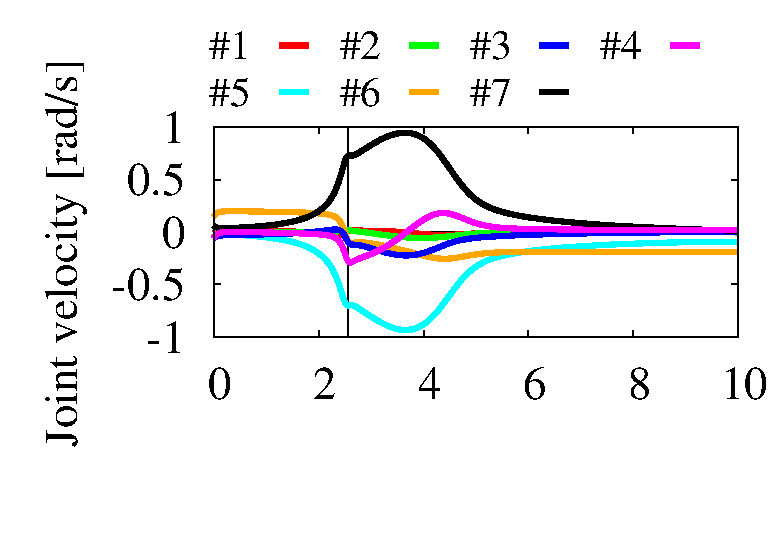
\includegraphics[width=1.0\linewidth]{fig/chapter4/inspection/singularity/SAMPLE/U01_joint_velo.eps}
  \end{minipage}
  \begin{minipage}[t]{0.40\linewidth}
    \centering
    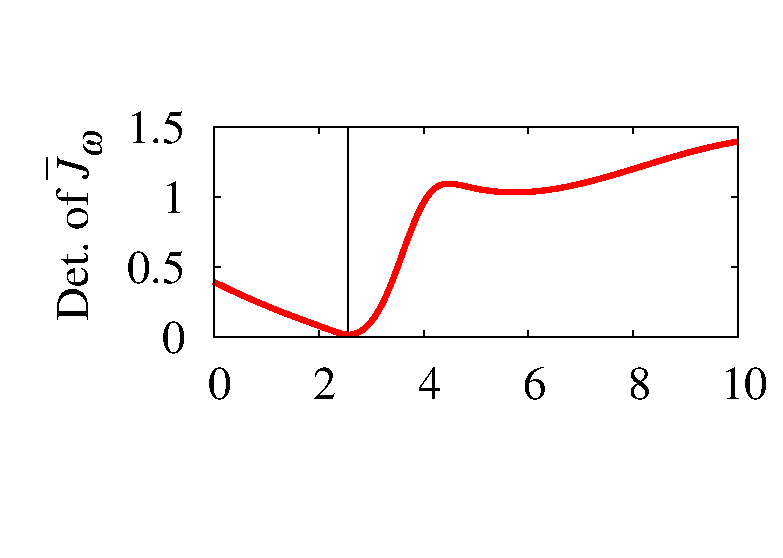
\includegraphics[width=1.0\linewidth]{fig/chapter4/inspection/singularity/SAMPLE/U16_determinant_Gw.eps}
  \end{minipage}\\
  \vspace{-5mm}
  \begin{minipage}[t]{0.40\linewidth}
    \centering
    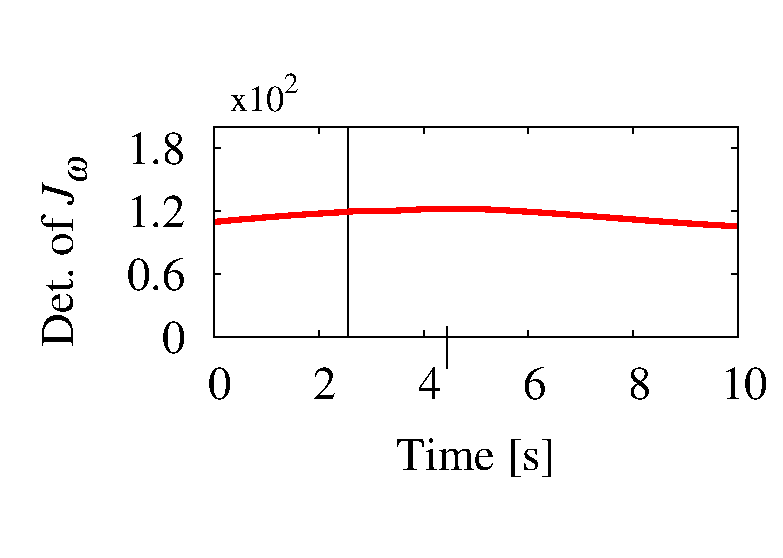
\includegraphics[width=1.0\linewidth]{fig/chapter4/inspection/singularity/SAMPLE/U14_determinant_Jw.eps}
  \end{minipage}
  \begin{minipage}[t]{0.40\linewidth}
    \centering
    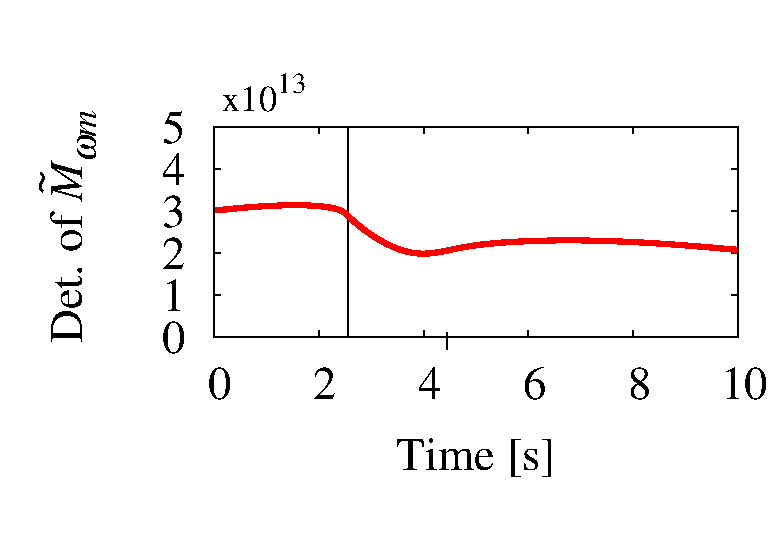
\includegraphics[width=1.0\linewidth]{fig/chapter4/inspection/singularity/SAMPLE/U15_determinant_Mwm.eps}
  \end{minipage}
  \caption{An example of the algorithmic singularity within the proposed method.}
  \label{fig:RES_SIN}
\end{figure}
% ---------------------------------------------------------------------
%
In the graphs, the vertical line represents the time instant when
the manipulator is passing  near a singularity whereby
$\det(\bar{\bm{J}}_{\omega_{e}}\bar{\bm{J}}_{\omega_{e}}^{T})$ approaches zero but the other two 
determinants,  $\mathrm{det}(\bm{J}_{\omega_{e}}\bm{J}_{\omega_{e}}^{T})$ and
$\mathrm{det}(\tbm{M}_{\omega m}\tbm{M}_{\omega m}^{T})$, do not. %  as shown in \fig{RES_SIN}.
Hence, this singularity can be recognized as an algorithmic one.
From the joint velocity graphs it is seen that near the singularity, 
Joints 5 and 7 rotate in opposite directions with high  joint rates.
This type of behavior is observed at singularities of the Euler angles \cite{Taki2013}
as well as at wrist singularities \cite{Aboaf1987}.

From our observation, it seems that such algorithmic  singularities do not occur frequently.
But nevertheless, we will show that singularity treatment techniques such as  the DLS and 
Singularity Consistent methods, can be effective w.r.t.\ algorithmic singularities.

%%%%%%%%%%%%%%%%%%%%%%%%%%%%%%%%%%%%%%%%%%%%%%%%%%%%%%%%%%%%%%%%%%%%%%%%%
\subsection{Singularity treatment with the Damped Least-Squares inverse}
\label{sec:SIN_DLS}
%%%%%%%%%%%%%%%%%%%%%%%%%%%%%%%%%%%%%%%%%%%%%%%%%%%%%%%%%%%%%%%%%%%%%%%%%
Originally, the DLS generalized inverse is obtained by  adding damping factors to the  denominators
in \eq{JP_SVD} to suppress high  joint rates.  We resume, however, to a DLS inverse that 
is obtained with a so-called  numerical filtering technique \cite{Chiaverini1997}. This approach can alleviate  
the problem of large errors. Accordingly, 
the generalized inverse of $\bar{\bm{J}}_{\omega_{e}}$ is obtained in the following form:
%
% ---------------------------------------------------------------------
\begin{align}
  \bar{\bm{J}}_{\omega_{e}}^{\#} = \bar{\bm{J}}_{\omega_{e}}^{T}\Big(\bar{\bm{J}}_{\omega_{e}}\bar{\bm{J}}_{\omega_{e}}^{T} +
  \lambda^{2}\bm{u}_{3}\bm{u}_{3}^{T}\Big)^{-1}\label{eq:INV_DAMPED}
\end{align}
% ---------------------------------------------------------------------
%
where  $\lambda$ is a damping factor,
$\bm{u}_{3}\R{3}$ is the left singular vector associated with the minimum singular value $\sigma_{3}$,
$(\circ)^{\#}$ represents the DLS inverse. 
%By replacing the pseudoinverse solution with the DLS one,we can deal with the singularity problem.
Further on, through SVD \eq{INV_DAMPED} can be rewritten as:
%
% ---------------------------------------------------------------------
\begin{align}
  \bar{\bm{J}}_{\omega_{e}}^{\#} = \sum_{i = 1}^{2}\frac{1}{\sigma_{i}}\bm{v}_{i}\bm{u}_{i}^{T} +
  \frac{\sigma_{3}}{\sigma_{3}^{2} + \lambda^{2}}\bm{v}_{3}\bm{u}_{3}^{T}\label{eq:INV_SVD}
\end{align}
% ---------------------------------------------------------------------
%
where $\sigma_{1} \geq \sigma_{2} \geq \sigma_{3}$ are the singular values of $\bar{\bm{J}}_{\omega_{e}}$ and
$\bm{u}_{i}\R{3}$, $\bm{v}_{i}\R{7}$ are the associated left and right singular vectors.
Compared with \eq{JP_SVD}, it can be seen that the DLS inverse with numerical filtering
is characterized by inserting  a damping factor  only into the last term, with the 
minimum singular value. Hence, compared to the original DLS inverse
which adds damping into all terms, the error of the solution can be reduced \cite{Chiaverini1997}.
%
% ---------------------------------------------------------------------
\begin{figure}[t]
  \centering
  \begin{minipage}[h]{0.40\linewidth}
    \centering
    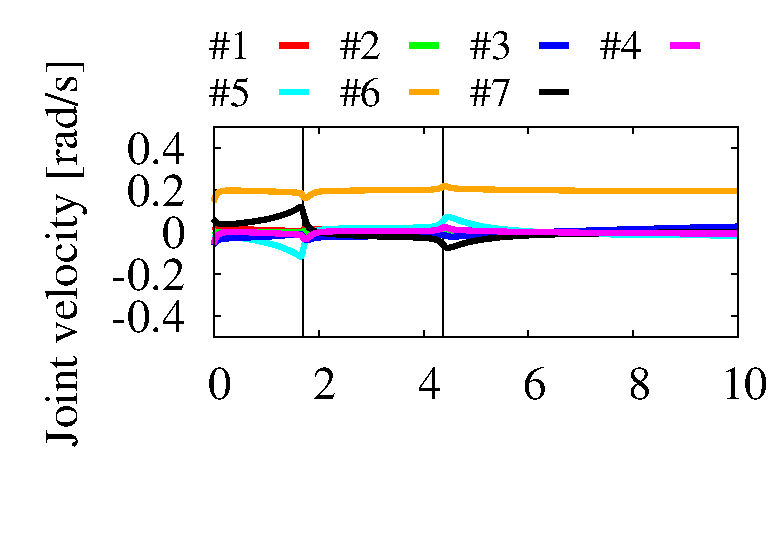
\includegraphics[width=1.0\linewidth]{fig/chapter4/inspection/singularity/DLS/U01_joint_velo.eps}
  \end{minipage}
  \begin{minipage}[h]{0.40\linewidth}
    \centering
    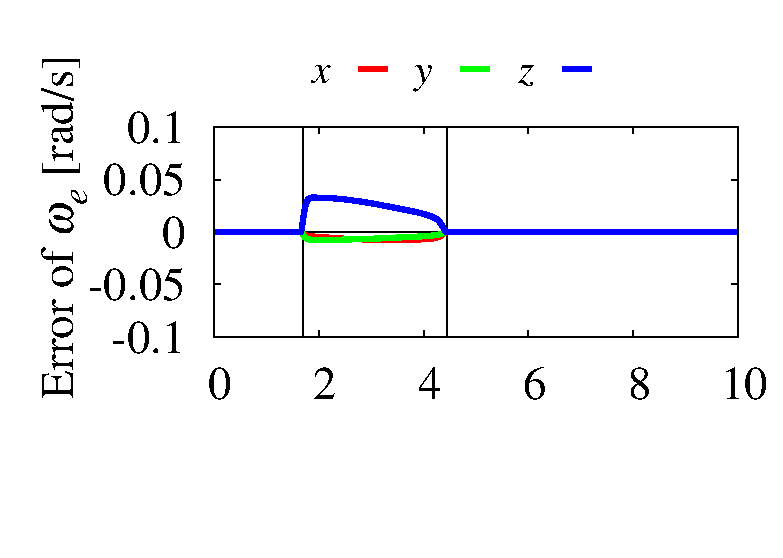
\includegraphics[width=1.0\linewidth]{fig/chapter4/inspection/singularity/DLS/U20_EE_vel_error.eps}
  \end{minipage}\\
  \vspace{-7mm}
  \begin{minipage}[h]{0.40\linewidth}
    \centering
    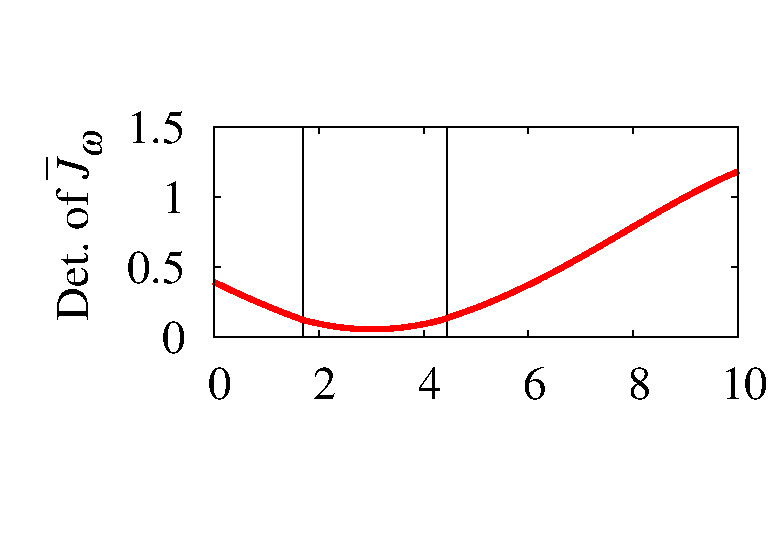
\includegraphics[width=1.0\linewidth]{fig/chapter4/inspection/singularity/DLS/U16_determinant_Gw.eps}
  \end{minipage}
  \begin{minipage}[h]{0.40\linewidth}
    \centering
    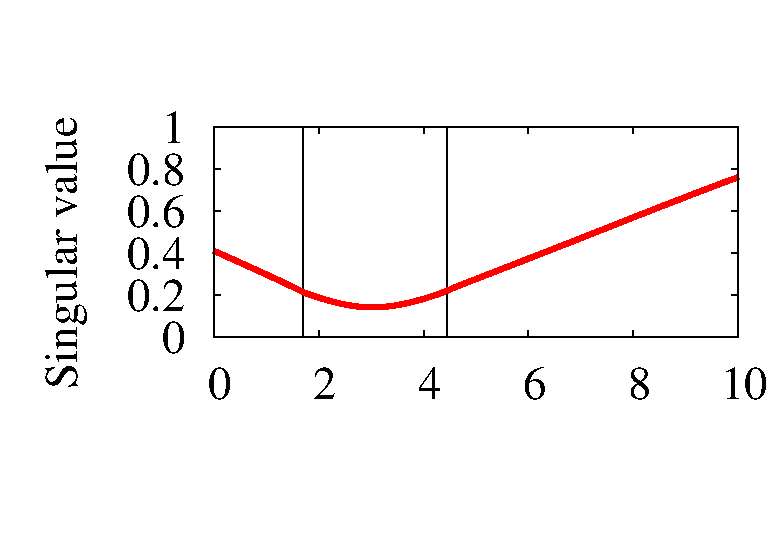
\includegraphics[width=1.0\linewidth]{fig/chapter4/inspection/singularity/DLS/U18_minimal_singular_value.eps}
  \end{minipage}\\
  \vspace{-7mm}
  \begin{minipage}[h]{0.40\linewidth}
    \centering
    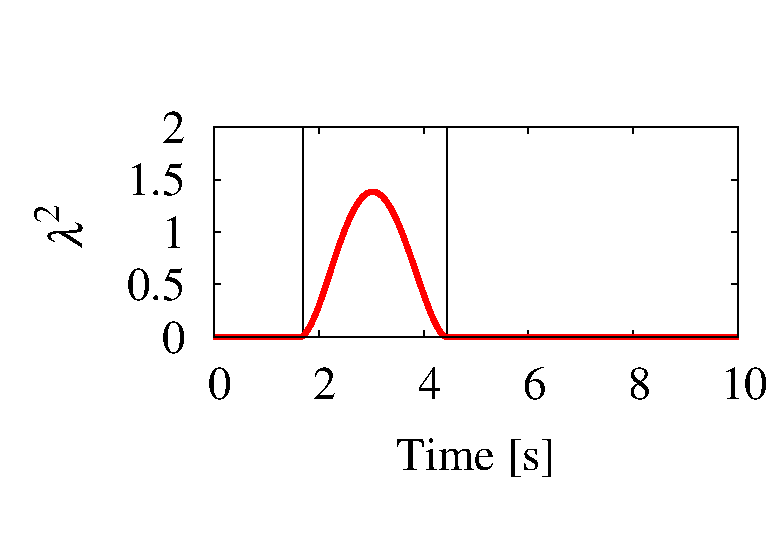
\includegraphics[width=1.0\linewidth]{fig/chapter4/inspection/singularity/DLS/U19_interpolation.eps}
  \end{minipage}
  \begin{minipage}[h]{0.40\linewidth}
    \centering
    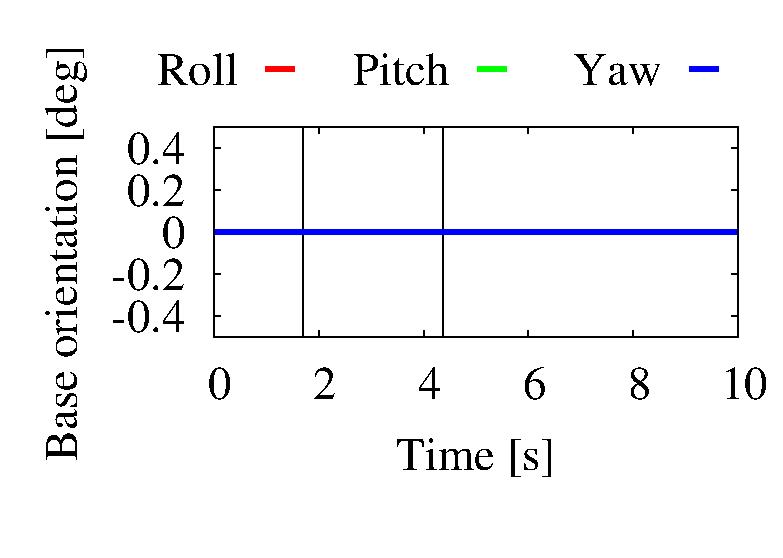
\includegraphics[width=1.0\linewidth]{fig/chapter4/inspection/singularity/DLS/X02_Base_Orientation.eps}
  \end{minipage}
  \caption{Simulation results under the damped least-squares inverse with numerical filtering.}
  \label{fig:RES_DLS}
\end{figure}
% ---------------------------------------------------------------------
%
Based on \cite{Chiaverini1994},
the damping factor is obtained as follows:
%
% ---------------------------------------------------------------------
\begin{align}
   \lambda^{2} &= \begin{cases} 0 & \varepsilon < \sigma_{3} \\
    (1 - \frac{2\sigma^{2}_{3}}{\varepsilon^{2}} + \frac{\sigma_{3}^{4}}{\varepsilon^{4}})\lambda_{max}^{2}
   & \sigma_{3} \leq \varepsilon\label{eq:damper}
  \end{cases}
\end{align}
% ---------------------------------------------------------------------
%
where  $\varepsilon$ defines the singular region,
which is introduced in the neighborhood of the singularity,
$\lambda_{max}$ sets the maximum value of the damping factor.
Note that we added an additional term, the $\sigma_{3}^{4}$ related term, 
into \eq{damper} to obtain a smooth transition at the border of the singular region.
%The original one did not consider the continuity at the first differential in 
%terms of $\sigma_{3}$.

The performance of the DLS inverse for this controller
is verified via numerical simulation.
The simulation conditions are the same as in \sec{PROBLEM}.
The singular region is defined by $\varepsilon = 0.2$ and
the maximum damping value set at $\lambda_{max}^{2} = 2$.
The results are displayed in \fig{RES_DLS}.
In the graphs, the singular region is indicated by the two vertical lines 
($1.71\unit{s} \leq t \leq 4.18\unit{s}$). From the results it is apparent that
the growth of the joint velocity has been successfully suppressed through the damping factor.
However, an end-effector tracking error can be observed within the singular region.
This is caused by the damping factor, as already explained. On the other hand,
the base attitude does not deviate, even within the singular region.


%%%%%%%%%%%%%%%%%%%%%%%%%%%%%%%%%%%%% HERE %%%%%%%%%%%%%%%%%%%%%%%%%%%%%%%%%%%%
\subsubsection{The Singularity Consistent method}
\label{sec:SIN_SC}
%%%%%%%%%%%%%%%%%%%%%%%%%%%%%%%%%%%%%%%%%%%%%%%%%%%%%%%%%%%%%%%%%%%%%%%%%
We will examine the possibility to make use of the Singularity Consistent (SC) method
for singularity treatment. It was clarified that the DLS method introduces an error
in the direction of motion since the singular direction, i.e.\ $\bm{v}_{3}$, has to 
be avoided. In contrast,
the SC method actively makes use of this direction and therefore, 
the manipulator can follow the direction of the desired end-effector velocity, correctly.
An error only appears in the speed along the path. If we consider a teleoperation task,
such an error is not a problem because the operator can modify the desired end-effector speed
according to the task conditions. Teleoperation under the SC method is discussed  in 
\cite{Tsumaki1997,Tsumaki1998}.

We will make use of natural motion \cite{Nenchev2007,Nenchev2010}, i.e.\ 
end-effector motion with velocity in proportion to
the determinant of the Jacobian matrix. There is no need to define a singular region then, and hence,
to switch the control input.

According to the SC method,  the inverse of $\bar{\bm{J}}_{\omega_{e}}$ can be obtained as follows:
%
% ---------------------------------------------------------------------
\begin{align}
  \bar{\bm{J}}_{\omega_{e}}^{+} &= b\sum_{i=1}^{3}\mu_{i}\bm{v}_{i}\bm{u}_{i}^{T}\label{eq:SC_INV}\\
  \mu_{i} &= \prod_{j=1, j\not = i}^{3}\sigma_{i}\label{eq:SC_SV}
\end{align}
% ---------------------------------------------------------------------
%
where $b$ is a constant scalar. From \eq{SC_SV},
we can see that $\mu_{1}$ and $\mu_{2}$ become small near the singularity,
because their values are proportional to the minimum singular value that approaches $0$ in the 
vicinity of the singularity. Hence, the $\bm{v}_{3}$ related term is actively used.

We verify the performance of this method through numerical simulation.
The simulation conditions are the same as in the DLS case. 
Empirically, the constant scalar was set to $b = 1.7$.
In addition, to avoid a large joint velocity obtained from the null-space term,
we multiply the term by the determinant of $\bar{\bm{J}}_{\omega_{e}}\bar{\bm{J}}_{\omega_{e}}^{T}$ as follows:
%
% ---------------------------------------------------------------------
\begin{align}
  \thd^{ref} = \bar{\bm{J}}_{\omega_{e}}^{+}\bm{\omega}_{e}^{ref} + 
k_{g}\mathrm{det}(\bar{\bm{J}}_{\omega_{e}}\bar{\bm{J}}_{\omega_{e}}^{T})\bm{P}(\bm{J}_{v_{w}}^{T})\Delta\bm{p}_{w}
\end{align}
% ---------------------------------------------------------------------
%
The simulation results are displayed in \fig{RES_SC}.
The results show that the rapid change of the joint velocity can be avoided.
In addition to this feature, it is seen that the end-effector  follows the desired 
velocity direction $y$, which is in contrast with the result from the DLS simulation.
Hence, adjustment of the speed is only needed by the operator under teleoperation.

%
% ---------------------------------------------------------------------
\begin{figure}[t]
  \centering
  \begin{minipage}[h]{0.40\linewidth}
    \centering
    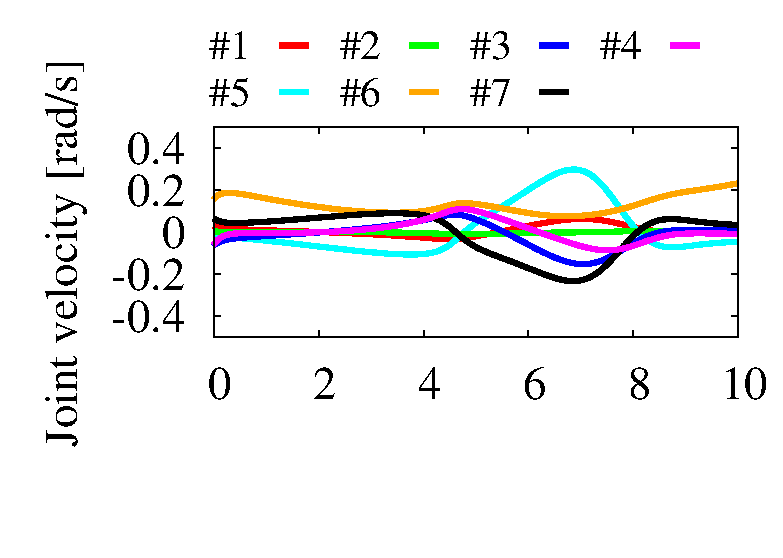
\includegraphics[width=1.0\linewidth]{fig/chapter4/inspection/singularity/SC/U01_joint_velo.eps}
  \end{minipage}
  \begin{minipage}[h]{0.40\linewidth}
    \centering
    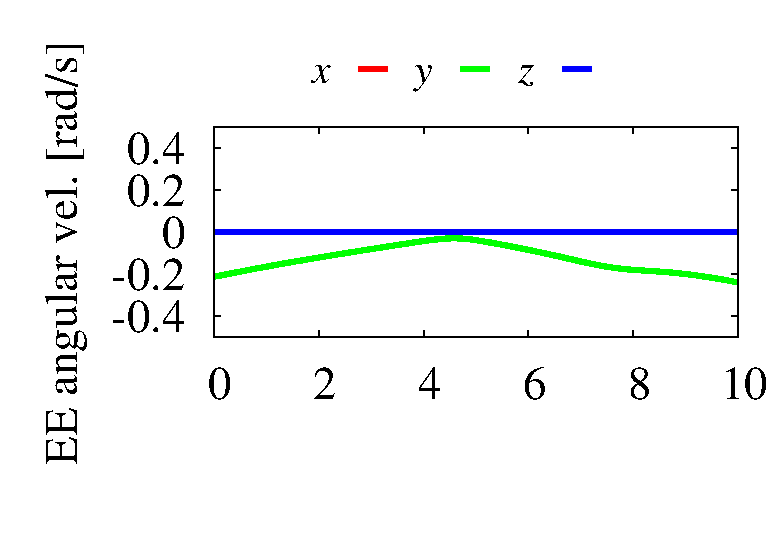
\includegraphics[width=1.0\linewidth]{fig/chapter4/inspection/singularity/SC/U08_end_tip_ang_vel.eps}
  \end{minipage}\\
  \vspace{-5mm}
  \begin{minipage}[h]{0.40\linewidth}
    \centering
    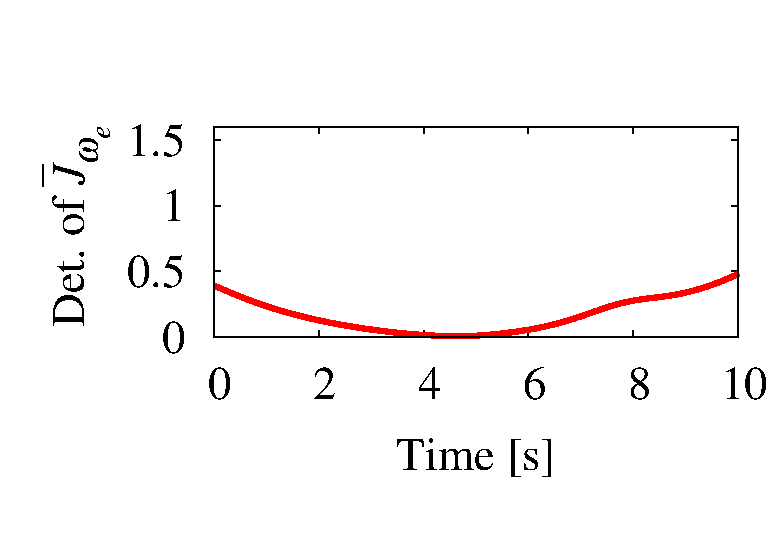
\includegraphics[width=1.0\linewidth]{fig/chapter4/inspection/singularity/SC/U16_determinant_Gw.eps}
  \end{minipage}
  \begin{minipage}[h]{0.40\linewidth}
    \centering
    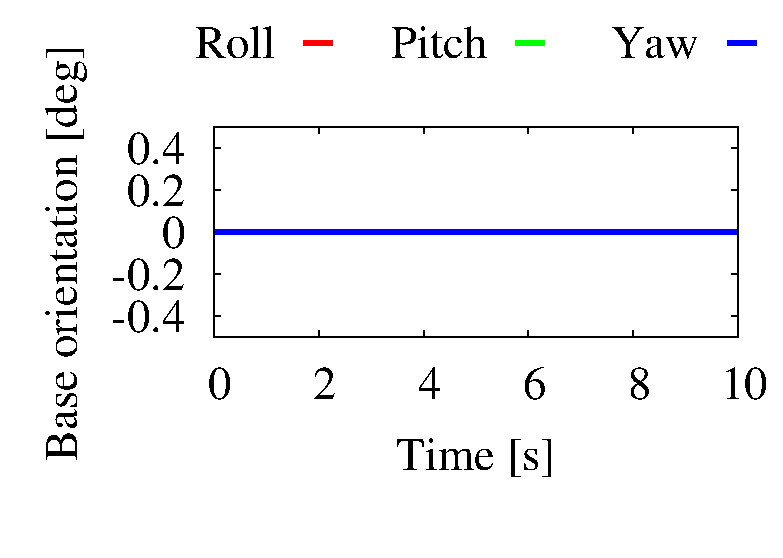
\includegraphics[width=1.0\linewidth]{fig/chapter4/inspection/singularity/SC/X02_Base_Orientation.eps}
  \end{minipage}
  \caption{Simulation results under the singularity consistent method.}
  \label{fig:RES_SC}
\end{figure}
% ---------------------------------------------------------------------
%



%%%%%%%%%%%%%%%%%%%%%%%%%%%%%%%%%%%%%%%%%%%%%%%%%%%%%
\section{Point-to-point positioning task}
%%%%%%%%%%%%%%%%%%%%%%%%%%%%%%%%%%%%%%%%%%%%%%%%%%%%%
As the second reactionless task,
we focus on point-to-point (PTP) positioning tasks of the end-effector.
PTP positioning tasks would be used several situation such as
pre-positioning task of the camera inspection, assembly and so on.
Among the several positioning tasks,
we restrict our attention to a specific subset of PTP tasks:
arm reconfiguration tasks wherein the hand does not hold an object.
It would be desirable to execute such tasks under reactionless motion control.

However,
this is impossible for arbitrary points since reactionless motions are quite restricted.
Nevertheless, reactionless motion can be useful if the PTP motion is planned appropriately.
One possibility is to combine two reactionless motions with a non-restricted PTP motion 
that induces the base disturbance.
This method was originally proposed in \cite{Yoshida1996};
it has been referred to as the \textit{3-Phase method} and
applied to a planar flexible base robots.
Note that despite the advantage of the method was
verified with a planar flexible base robots,
the cases of free-floating base robots and also
three-dimensional models have not been discussed before.
We verify the performance of this method with the three-dimensional free-floating robot.

%%%%%%%%%%%%%%%%%%%%%%%%%%%%%%%%%%%%%
\subsection{The 3-Phase method}
%%%%%%%%%%%%%%%%%%%%%%%%%%%%%%%%%%%%%

%
% ---------------------------------------------------------------------
\begin{figure}[t]
  \centering
  \begin{minipage}[h]{0.8\linewidth}
    \centering
    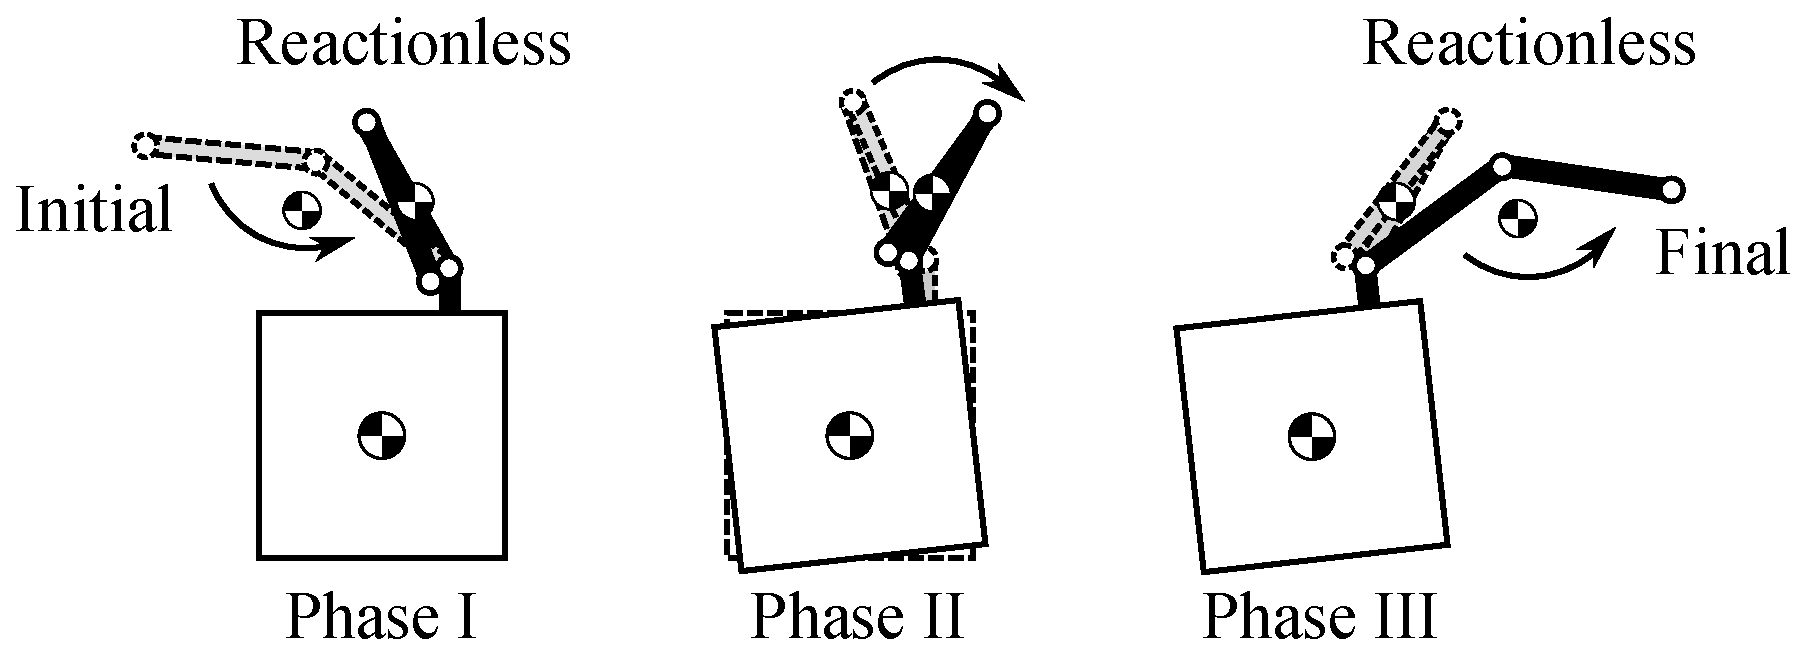
\includegraphics[width=1.0\linewidth]{fig/chapter4/PTP/motion.eps}
  \end{minipage}
  \caption{A motion obtained via the 3-Phase method.}
  \label{fig:3PHASE}
\end{figure}
% ---------------------------------------------------------------------
%
First, we review the 3-Phase method.
The 3-Phase method deals with the following issue:
find a joint path that connects specific initial and final configurations
with three sub-paths.
We divide a motion into three Phase, which are Phase I, II and III, according to the three sub-paths.
In Phase I and III,
reactionless motion is used.
In Phase II,
these two reactionless motion paths are connected via a joint path that is not reactionless.
% A graphical image of the 3-Phase method is depicted in \fig{3PHASE}.
The primary concern is how to determine the three sub-paths to obtain small base disturbance
during the PTP sub-paths in Phase II.
In \cite{Yoshida1996},
a folded arm configuration as shown in \fig{3PHASE} was employed in Phase II.
Using this configuration, the base disturbance can be reduced.
We provide a theoretical argument of reaction reduction with the folded configuration in what follows.
The coupling angular momentum, which is the base reaction with dimension of momentum,
can be represented in the following form:
%
% ---------------------------------------------------------------------
\begin{align}
  \tilde{\bm{M}}_{\omega m}\dot{\bm{\theta}} &= \Big\{\sum_{i = 1}^{n}\bm{I}_{i}\bm{J}_{\omega_{i}}\Big\}\dot{\bm{\theta}}~ + \notag\\
  &\Big\{\sum_{i=1}^{n}m_{i}[\bm{r}_{b \rightarrow i}^{\times}]\bm{J}_{v_{i}}\Big\}\thd -
  \Big\{m_{c}[\bm{r}_{b \rightarrow c}^{\times}]\bm{J}_{c}\Big\}\thd,
  \label{eq:CIM}
\end{align}
% ---------------------------------------------------------------------
%
It is apparent that the coupling angular momentum consists of three kinds of angular momentum.
The first term represents the angular momentum induced by
purely rotational motion of each link;
the second and third term are the angular momentum arising from the moment of the linear momentum
of each link and the CoM of the manipulator.
The coefficient matrix of the first term is related to the inertia tensor of the manipulator.
Hence, at the folded configuration,
this term becomes the smallest value.
On the other hand,
the second and third term are related to the CoM positions.
The base reaction related to these term also takes small amount
using the folded configuration,
because the distance along which the manipulator CoM moves becomes short,
as shown in \fig{3PHASE}.
In addition,
the norm of $\bm{r}_{b \rightarrow i}$ and $\bm{r}_{b \rightarrow c}$ become small value at the configuration.
Hence, the angular momentum related to the linear momentum of each link can be reduced.
For this reason, the folded configuration is used in Phase II.

% %
% % ---------------------------------------------------------------------
% \begin{figure}[t]
%   \centering
%   \begin{minipage}[h]{0.3\linewidth}
%     \centering
%     \includegraphics[width=1.0\linewidth]{fig/chapter4/PTP/Phase1.eps}
%     \footnotesize\par{\hspace{16mm}Phase I}
%   \end{minipage}
%   \hspace{4mm}
%   \begin{minipage}[h]{0.3\linewidth}
%     \centering
%     \includegraphics[width=1.0\linewidth]{fig/chapter4/PTP/Phase2.eps}
%     \footnotesize\par{Phase II}
%   \end{minipage}
%   \begin{minipage}[h]{0.245\linewidth}
%     \centering
%     \includegraphics[width=1.0\linewidth]{fig/chapter4/PTP/Phase3.eps}
%     \footnotesize\par{\vspace{-0.7mm}Phase III}
%   \end{minipage}
%   \caption{A motion obtained via the 3-Phase method.}
%   \label{fig:3PHASE}
% \end{figure}
% % ---------------------------------------------------------------------
% %



%%%%%%%%%%%%%%%%%%%%%%%%%%%%%%%%%%%%%%%%%%%%%%%%%%%%%
\subsection{Verification via numerical simulations}
%%%%%%%%%%%%%%%%%%%%%%%%%%%%%%%%%%%%%%%%%%%%%%%%%%%%%
%
% ---------------------------------------------------------------------
\begin{figure}[t]
  \centering
  \begin{minipage}[h]{0.4\linewidth}
    \centering
    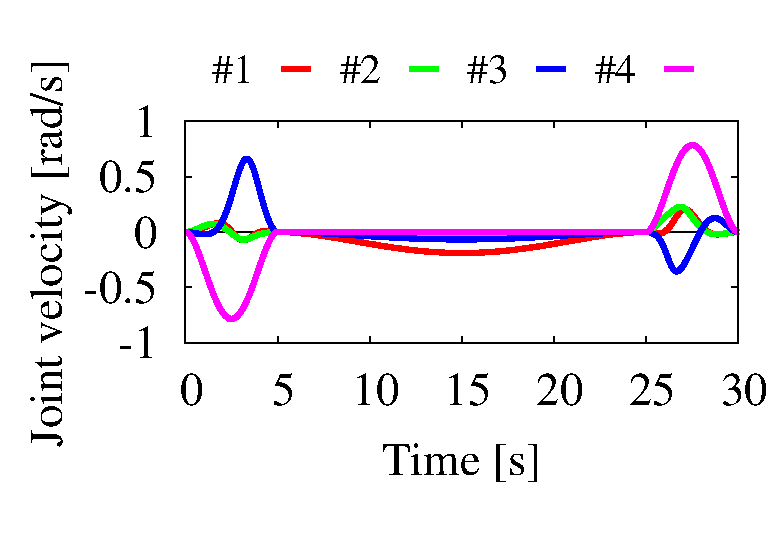
\includegraphics[width=1.0\linewidth]{fig/chapter4/PTP/3phase/U01_joint_velo_1-4.eps}
    \footnotesize\par{(a)}
  \end{minipage}
  \begin{minipage}[h]{0.4\linewidth}
    \centering
    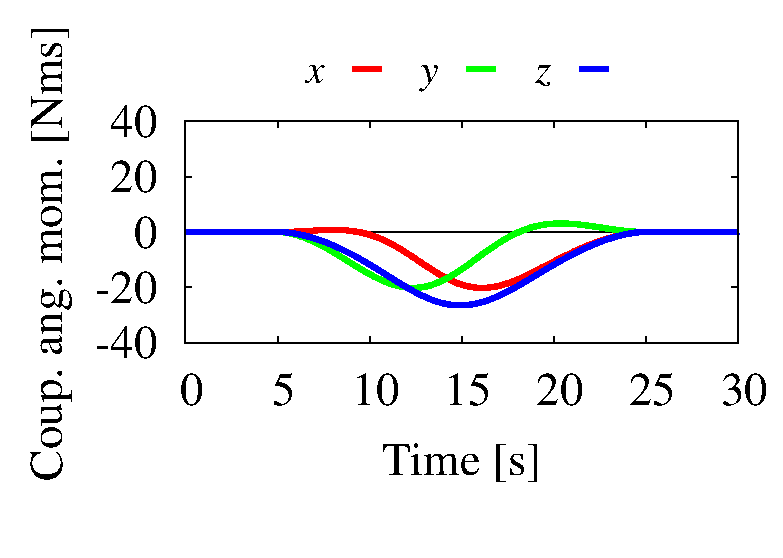
\includegraphics[width=1.0\linewidth]{fig/chapter4/PTP/3phase/U04_coup_ang_mom.eps}
    \footnotesize\par{(b)}
  \end{minipage}
  \caption{The simulation results under the 3-phase method:
  (a) the joint velocity and (b) the coupling angular momentum.}
  \label{fig:RES_3PHASE}
\end{figure}
% ---------------------------------------------------------------------
%
We verify the performance of the 3-Phase method via numerical simulations,
compared with several conventional controllers.
The initial configuration is $[-20~-40~0~-60~180~180~0]^{T}\unit{deg}$;
the final one is $[-120~50~0~-60~180~180~0]^{T}\unit{deg}$.
Note that these two configurations cannot be linked via reactionless motion.
The motion in Phase I is obtained from the initial configuration toward
a folded configuration (FA-1).
Phase III is determined as a reversed (reactionless) motion starting from the final configuration toward
other folded configuration (FA-2).
These two reactionless motions are obtained as the second term in \eq{RL_POS} as follows:
%
% ---------------------------------------------------------------------
\begin{align}
  \thd^{ref} &= \frac{\dot{\theta}_{4}^{ref}(t)}{n_{4}}\bmat{\bm{n} \\ \bm{0}}\\
  \dot{\theta}_{4}^{ref}(t) &= \dot{\theta}_{4}^{des}(t) + k\Delta\theta_{4}(t)
  \label{eq:PS_MOTION}
\end{align}
% ---------------------------------------------------------------------
%
where $n_{4}$ is the forth element of $\bm{n}$,
$\theta_{4}(t)^{des}$ is the desired trajectory of joint 4;
$\Delta\theta_{4}(t) = \theta_{4}^{des}(t) - \theta_{4}$ is the tracking error.
$k$ is a feedback gain.
The two folded configurations are distinct and uniquely defined as resultant configurations
along the respective reactionless motion, wherein $\theta_{4} = -\pi\unit{rad}$.
In Phase I and III,
the motions were executed in $5\unit{s}$,
and Phase II in $20\unit{s}$.

For the comparison,
the same positioning task was executed under the joint space interpolation with straight line (JS-C),
the inverse Jacobian controller (IJ-C) and the transposed Jacobian controller (TJ-C).
For the task space controllers (IJ and TJ-C),
the final condition was set to the final position of the end-effector in the 3-Phase method as
$[-1.7~0.45~1.7]^{T}\unit{m}$.
The three controllers were executed in $30\unit{s}$.
Note that orientation of the end-effector is not considered for the sake of simplicity.
Hence, only the positioning subchain was driven.

First, we show the results obtained in the 3-Phase method in \fig{RES_3PHASE}.
From the results,
the joint motion can be smoothly obtained and only Phase II introduced the coupling angular momentum.
%
% ---------------------------------------------------------------------
\begin{figure}[t]
  \centering
  \begin{minipage}[h]{0.3\linewidth}
    \centering
    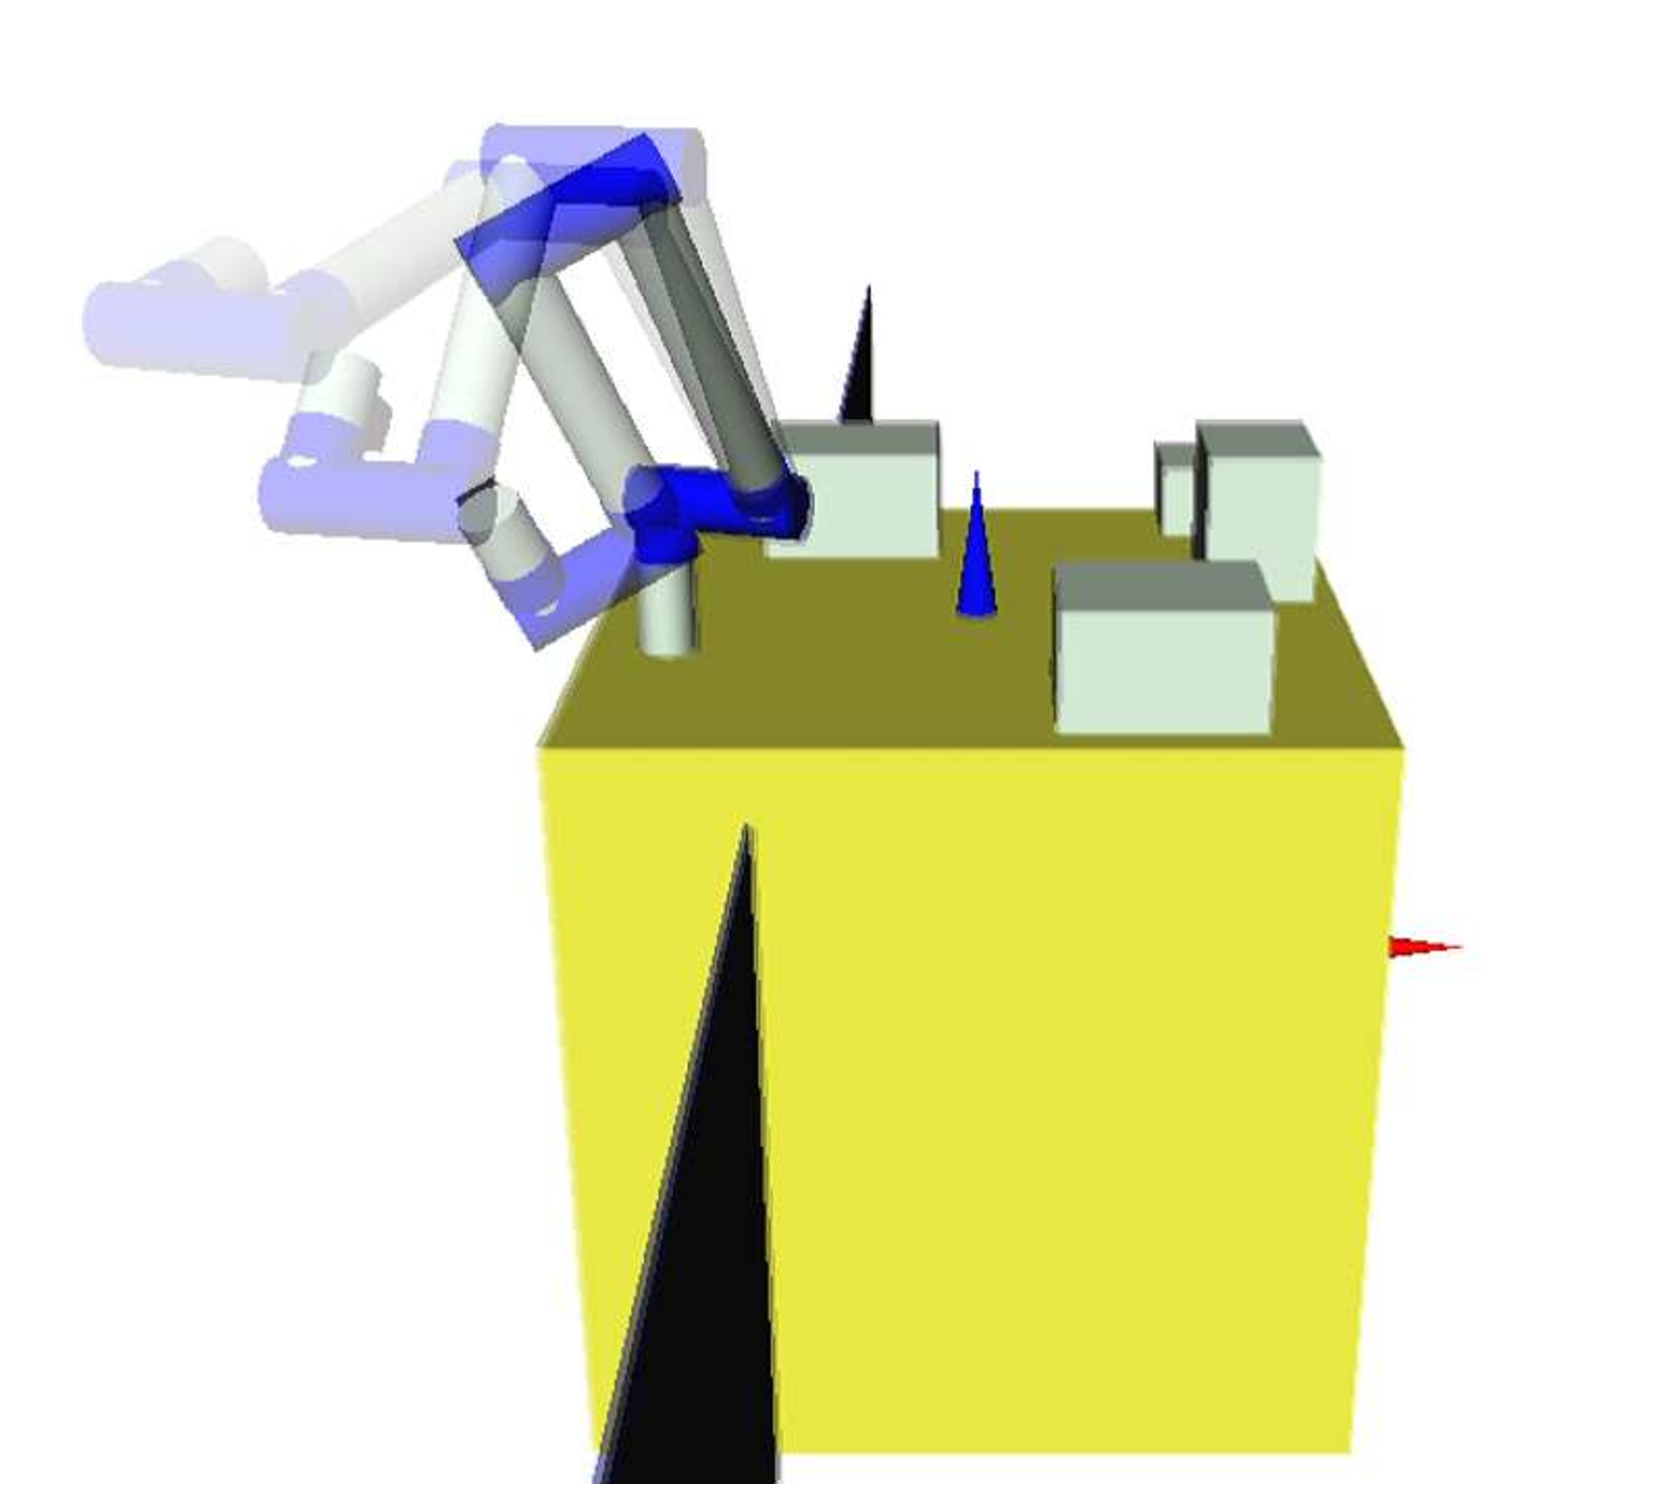
\includegraphics[width=1.0\linewidth]{fig/chapter4/PTP/phase1.eps}
    \footnotesize\par{Phase I}
  \end{minipage}
  \begin{minipage}[h]{0.3\linewidth}
    \centering
    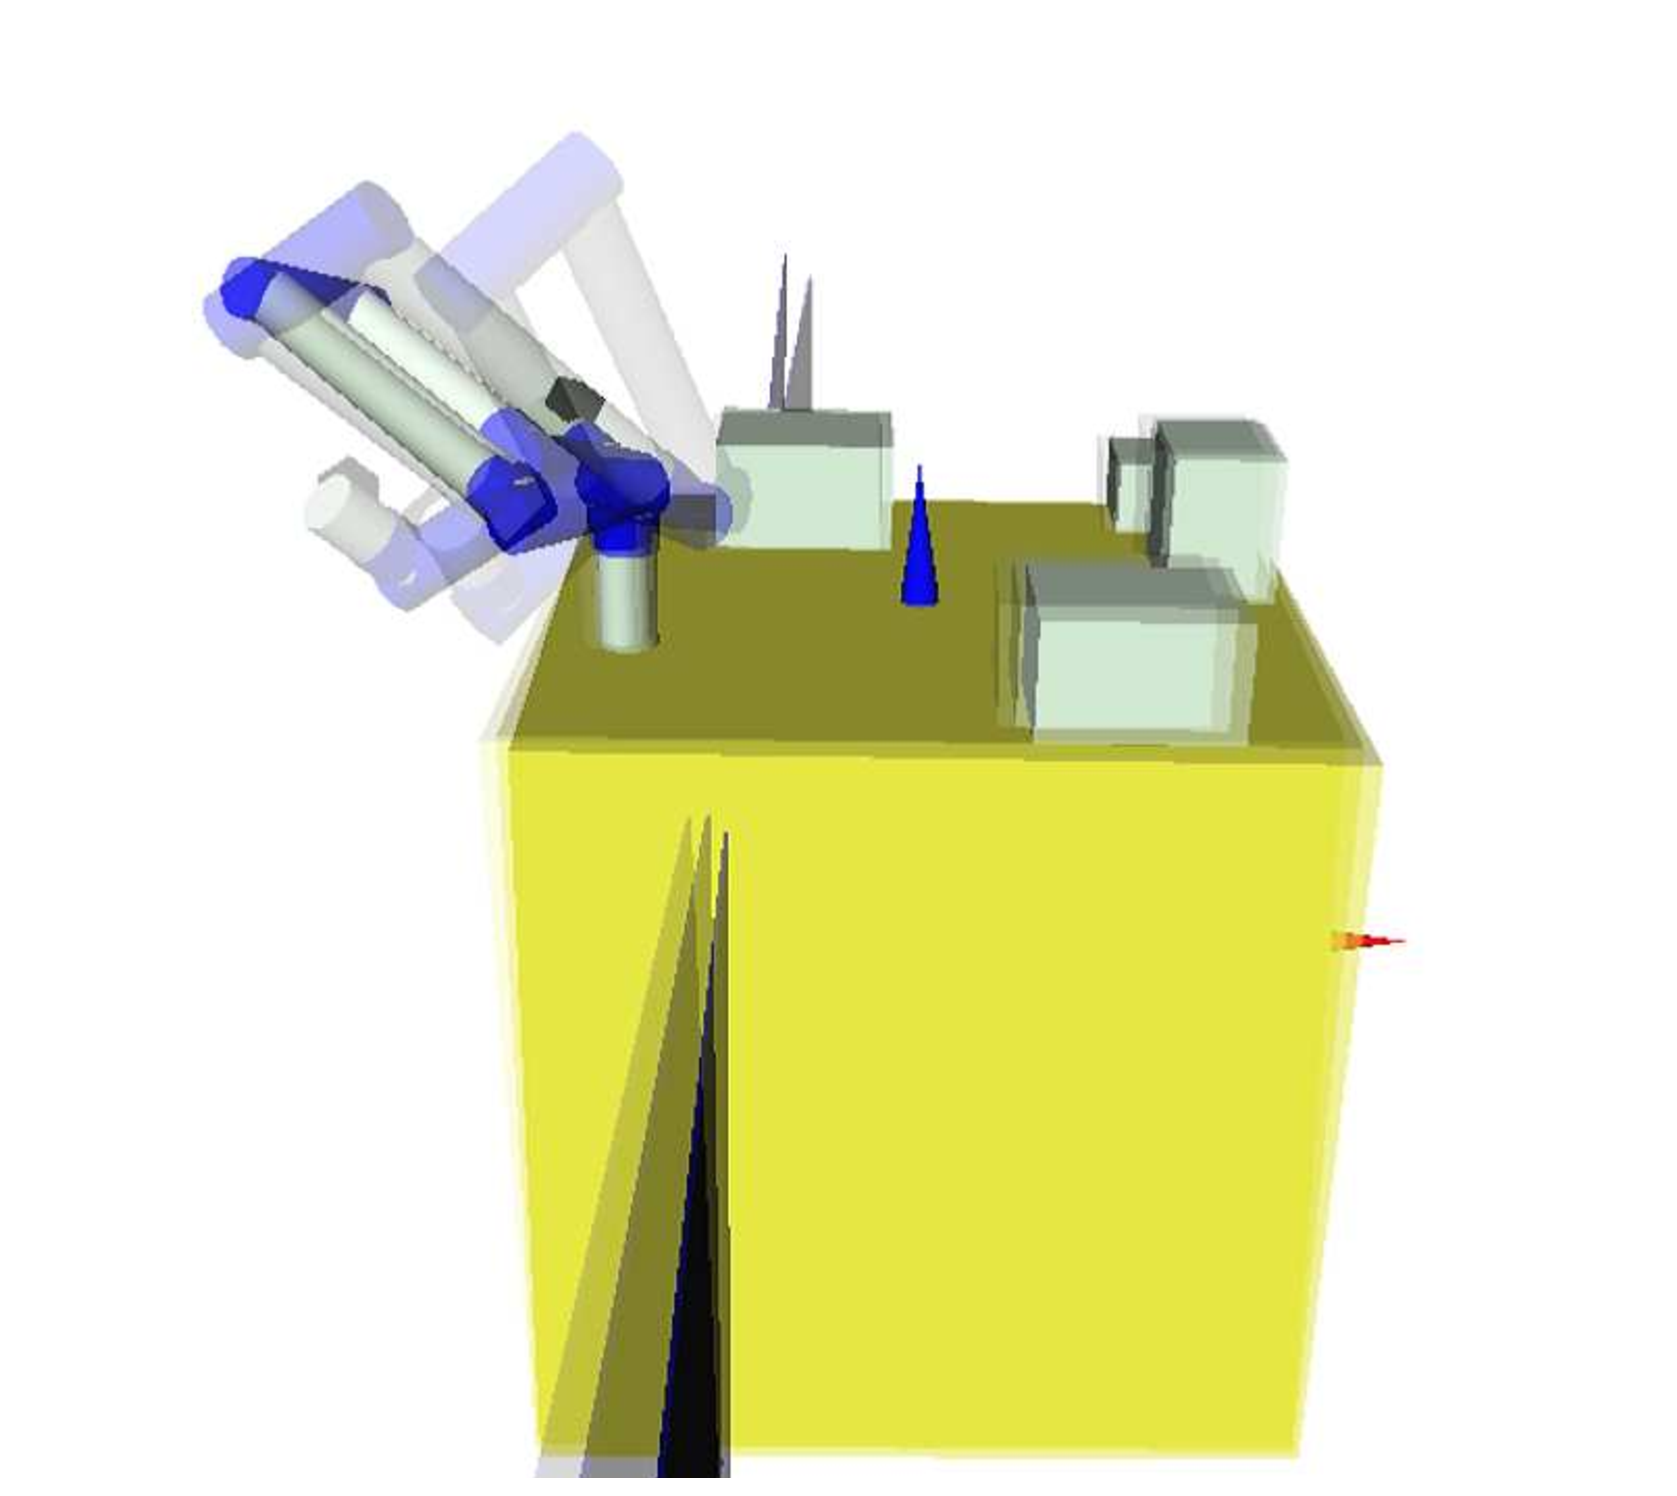
\includegraphics[width=1.0\linewidth]{fig/chapter4/PTP/phase2.eps}
    \footnotesize\par{Phase II}
  \end{minipage}
  \begin{minipage}[h]{0.3\linewidth}
    \centering
    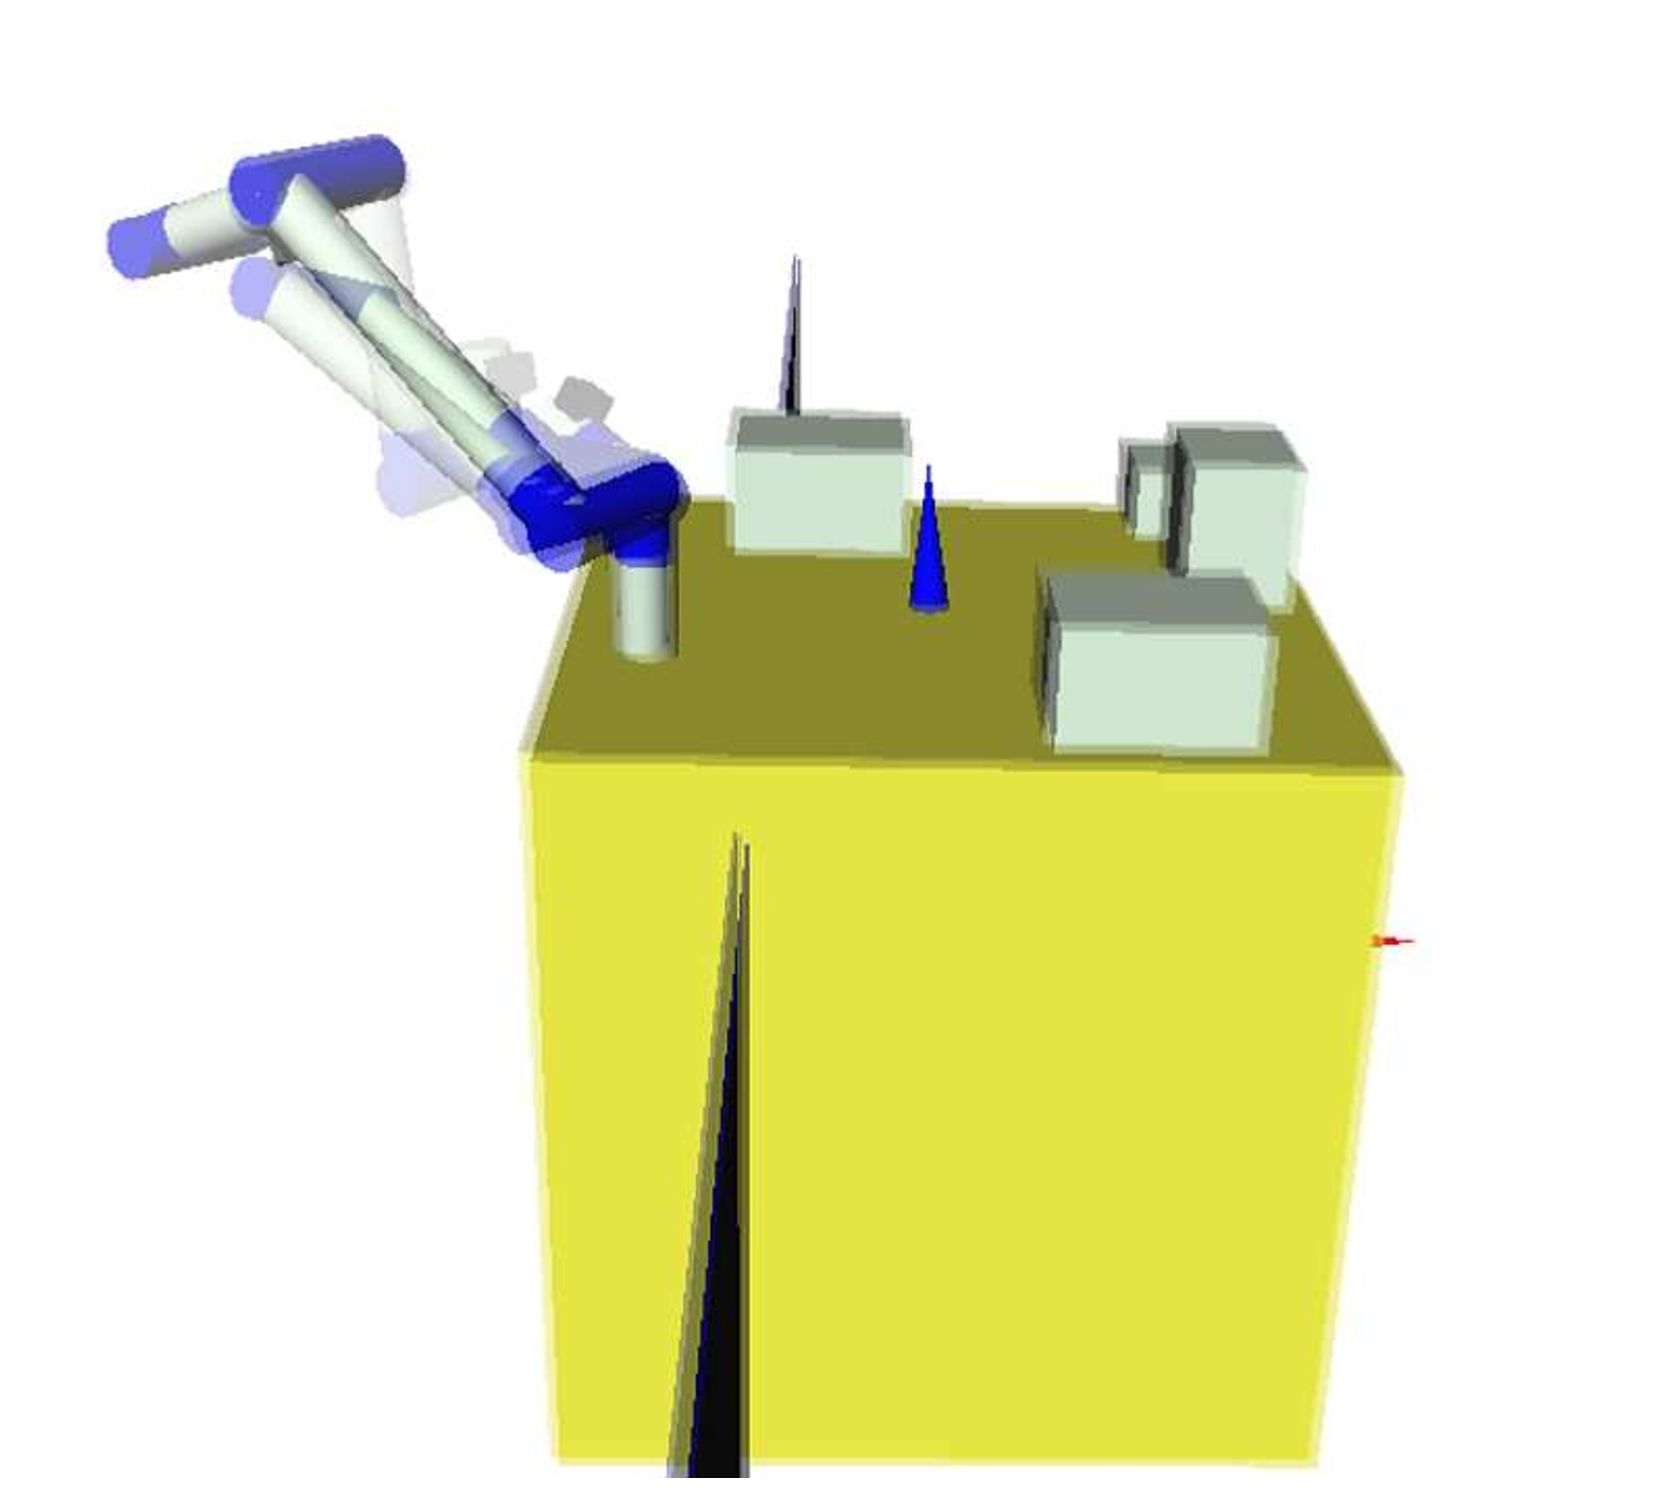
\includegraphics[width=1.0\linewidth]{fig/chapter4/PTP/phase3.eps}
    \footnotesize\par{Phase III}
  \end{minipage}
  \caption{The snapshot of the motion obtained via the 3-phase method.}
  \label{fig:SNAP_3PHASE}
\end{figure}
% ---------------------------------------------------------------------
%

To evaluate the performance in terms of the base reaction,
we compare the base attitude deviations under all methods.
The time profiles of the base attitude deviation are displayed in \tab{RES_COMP_PTP}.
The maximum deviation and the its ratio between the compared methods and the 3-phase are shown in \tab{RES_COMP_PTP}.
%
% ---------------------------------------------------------------------
\begin{figure}[t]
  \centering
  \begin{minipage}[h]{0.4\linewidth}
    \centering
    \includegraphics[width=1.0\linewidth]{fig/chapter4/PTP/3phase/X02_Base_Orientation.eps}
    \footnotesize\par{(a)}
  \end{minipage}
  \begin{minipage}[h]{0.4\linewidth}
    \centering
    \includegraphics[width=1.0\linewidth]{fig/chapter4/PTP/JS-C/X02_Base_Orientation.eps}
    \footnotesize\par{(b)}
  \end{minipage}
  \begin{minipage}[h]{0.4\linewidth}
    \centering
    \includegraphics[width=1.0\linewidth]{fig/chapter4/PTP/IJ-C/X02_Base_Orientation.eps}
    \footnotesize\par{(c)}
  \end{minipage}
  \begin{minipage}[h]{0.4\linewidth}
    \centering
    \includegraphics[width=1.0\linewidth]{fig/chapter4/PTP/TJ-C/X02_Base_Orientation.eps}
    \footnotesize\par{(d)}
  \end{minipage}
  \caption{The base attitude deviations under the all methods:
  (a) 3-phase method, (b) JS-C, (c) IJ-C and (d) TJ-C.}
  \label{fig:RES_COMP_PTP}
\end{figure}
% ---------------------------------------------------------------------
%
\begin{table}[t]
  \centering
  \caption{The maximum value of the base deviation.}
  \begin{tabular}[h]{c|c|c}\hline
    & Maximum deviation [deg] & Ratio \\\hline\hline
    3-Phase & 1.95 & 1.00\\\hline
    JS-C & 3.61 & 1.84 \\\hline
    IJ-C & 3.21 & 1.64 \\\hline
    TJ-C & 3.85 & 1.96 \\\hline
  \end{tabular}
  \label{tab:RES_COMP_PTP}
\end{table}

From the results,
it can be seen that the maximum deviation under the 3-phase method is
about two times smaller than that under the others.
Hence, we can conclude that the 3-phase method has a advantage in terms of the base reaction.



%%%%%%%%%%%%%%%%%%%%%%%%%%%%%%%%%%%%%%%%%%%%%%%%%%%%%%%%%%%%%%%%%%%%%%%%%%%%%%
\section{Deployment task}
%%%%%%%%%%%%%%%%%%%%%%%%%%%%%%%%%%%%%%%%%%%%%%%%%%%%%%%%%%%%%%%%%%%%%%%%%%%%%%
Finally, we discuss the possibility of reactionless motion control
under the deployment motion task from a stowed configurations.
When launching a free-floating space robot into orbit,
the manipulator has to be stowed to overcome several loads.
These configurations are referred to as the \textit{stowed configurations}.
An example is displayed in \fig{SNAP_DEPLOY} (upper left).
During on-orbit experiments,
deployment from the configuration has to be executed at least few times.
We propose reactionless motion control in the following two case:
(i) full reactionless deployment and
(ii) partial reactionless deployment.

%%%%%%%%%%%%%%%%%%%%%%%%%%%%%%%%%%%
\subsection{Full reactionless task}
%%%%%%%%%%%%%%%%%%%%%%%%%%%%%%%%%%%
First, we examine the possibility of a deployment task under fully reactionless condition.
For the sake of simplicity,
we only use the positioning subchain because the effect of wrist motion is relatively small
at this motion task.
As a result,
the DoF of reactionless motion becomes one due to considering only the positioning subchain.
Therefore,
the reactionless motion path is uniquely determined according to a initial configuration.
The final (deployed) configuration can be selected as any configurations along the reactionless path.
The selection will depend upon the subsequent task.
The benefit is that the speed/acceleration along the reactionless path connecting the two configurations
can be set freely that allows for a very time-efficient deployment.

We define the candidates for the stowed configuration of the our manipulator model as follows:
%
% ---------------------------------------------------------------------
\begin{align}
  \th_{st} = \{\th\R{7} | \theta_{i} = \pm \pi/2, \theta_{j} = 0,\pm \pi, \forall \theta_{k}\}\notag\\
  (i = 1,2,~j = 3~\mathrm{to}~5,~k = 6,7)
\end{align}
% ---------------------------------------------------------------------
%
Among them, we pick up a configuration that is well-conditioned for the reactionless motion:
$[\pi/2~-\pi/2~0~-\pi~\pi~\pi~0]^{T}\unit{rad}$.
Snapshots of the deployment sequence during $30\unit{s}$ are shown in \fig{SNAP_DEPLOY}.
The motion was obtained via \eq{PS_MOTION}
with the constant speed of joint 4: $\dot{\theta}_{4}^{des} = 0.183\unit{rad/s}$.
%
% ---------------------------------------------------------------------
\begin{figure}[t]
  \centering
  \begin{minipage}[h]{0.28\linewidth}
    \includegraphics[width=1.0\linewidth]{fig/chapter4/deployment/01.eps}
      \centering
      \par\footnotesize{$t = 0.0~\mathrm{s}$}
  \end{minipage}
  \begin{minipage}[h]{0.28\linewidth}
    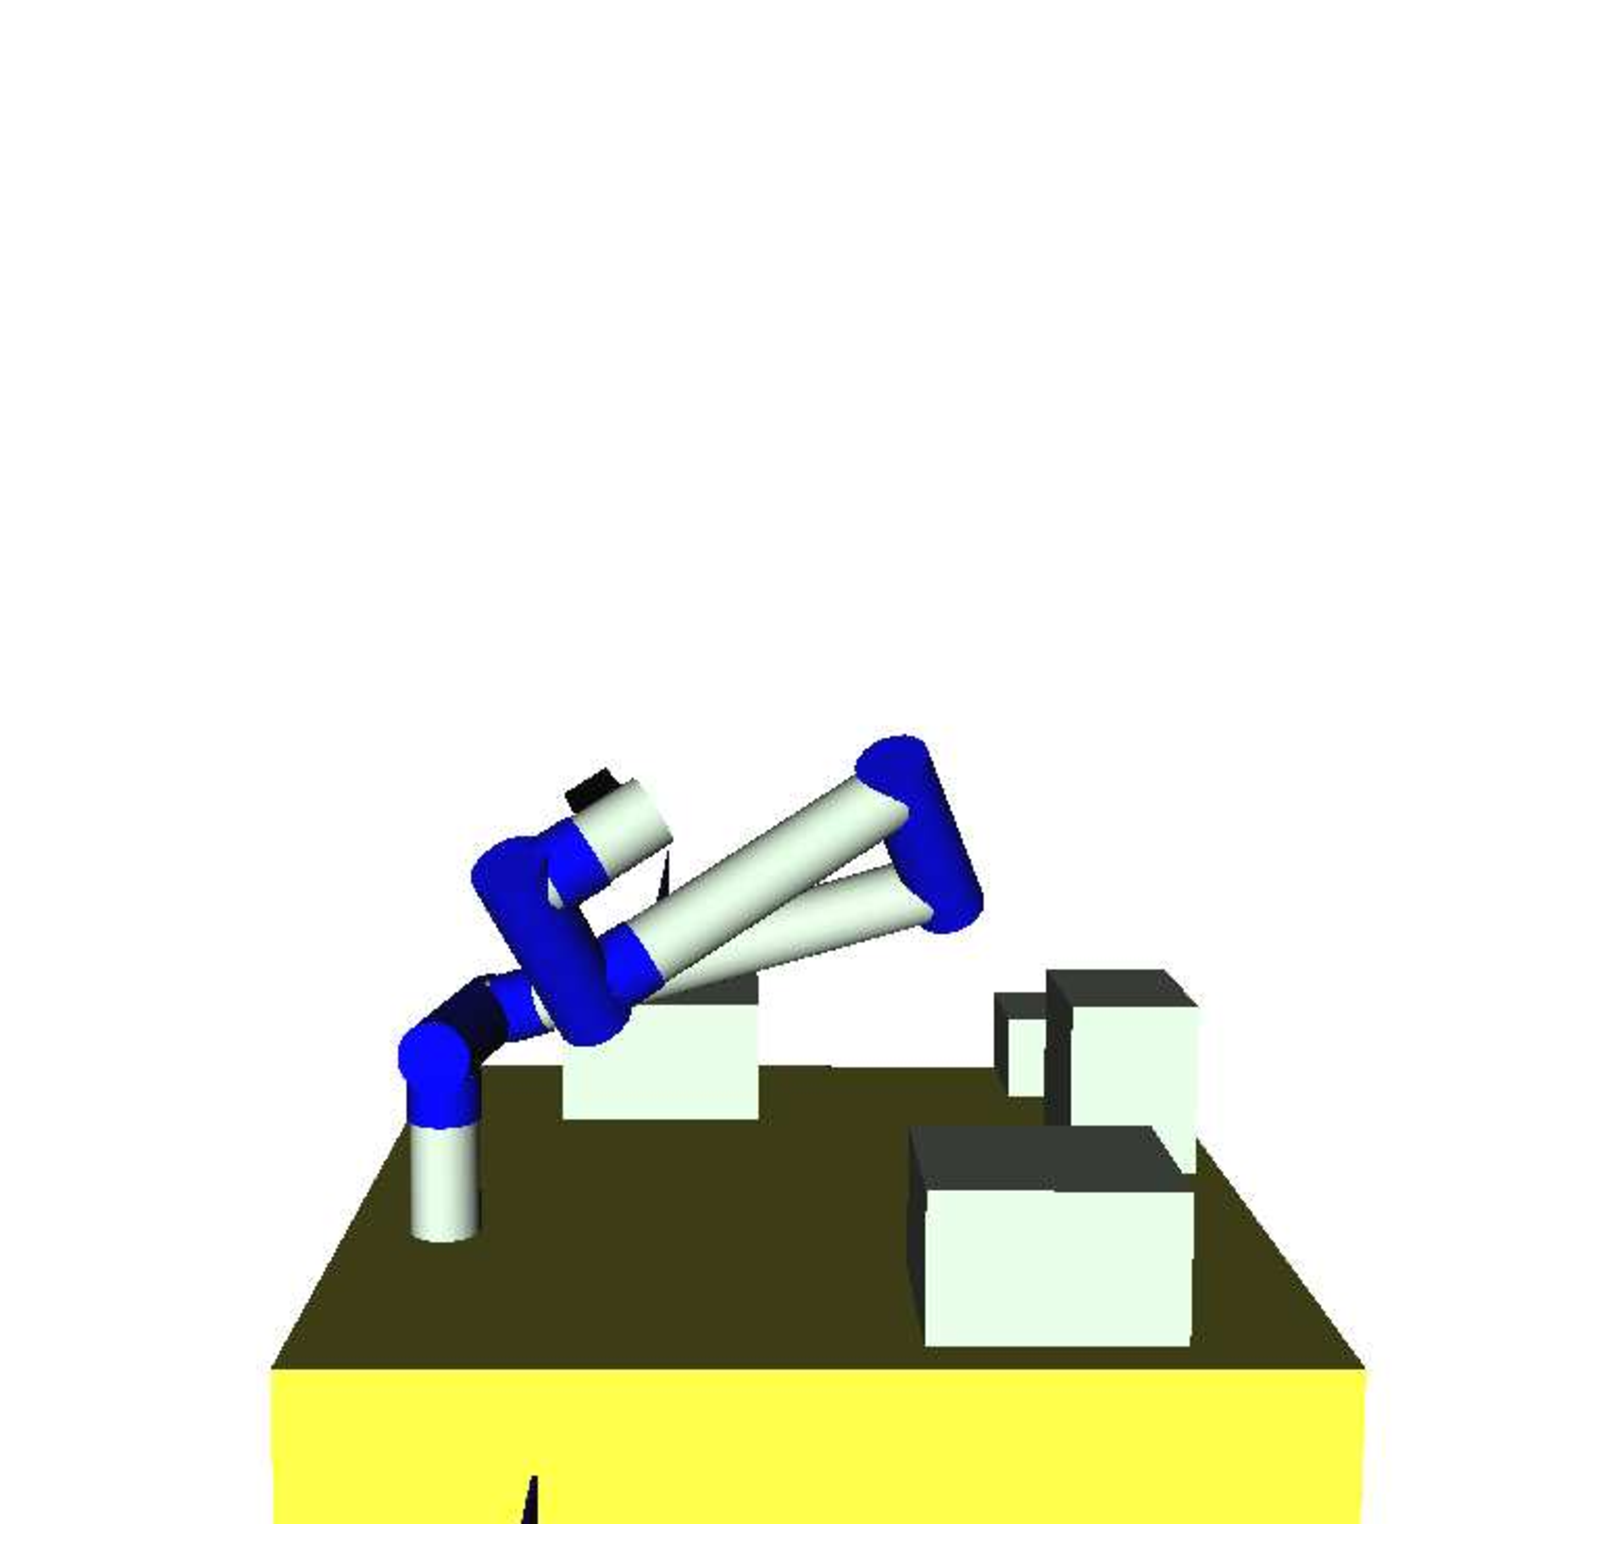
\includegraphics[width=1.0\linewidth]{fig/chapter4/deployment/02.eps}
    \centering
    \par\footnotesize{$t = 9.0~\mathrm{s}$}
  \end{minipage}
  \begin{minipage}[h]{0.28\linewidth}
    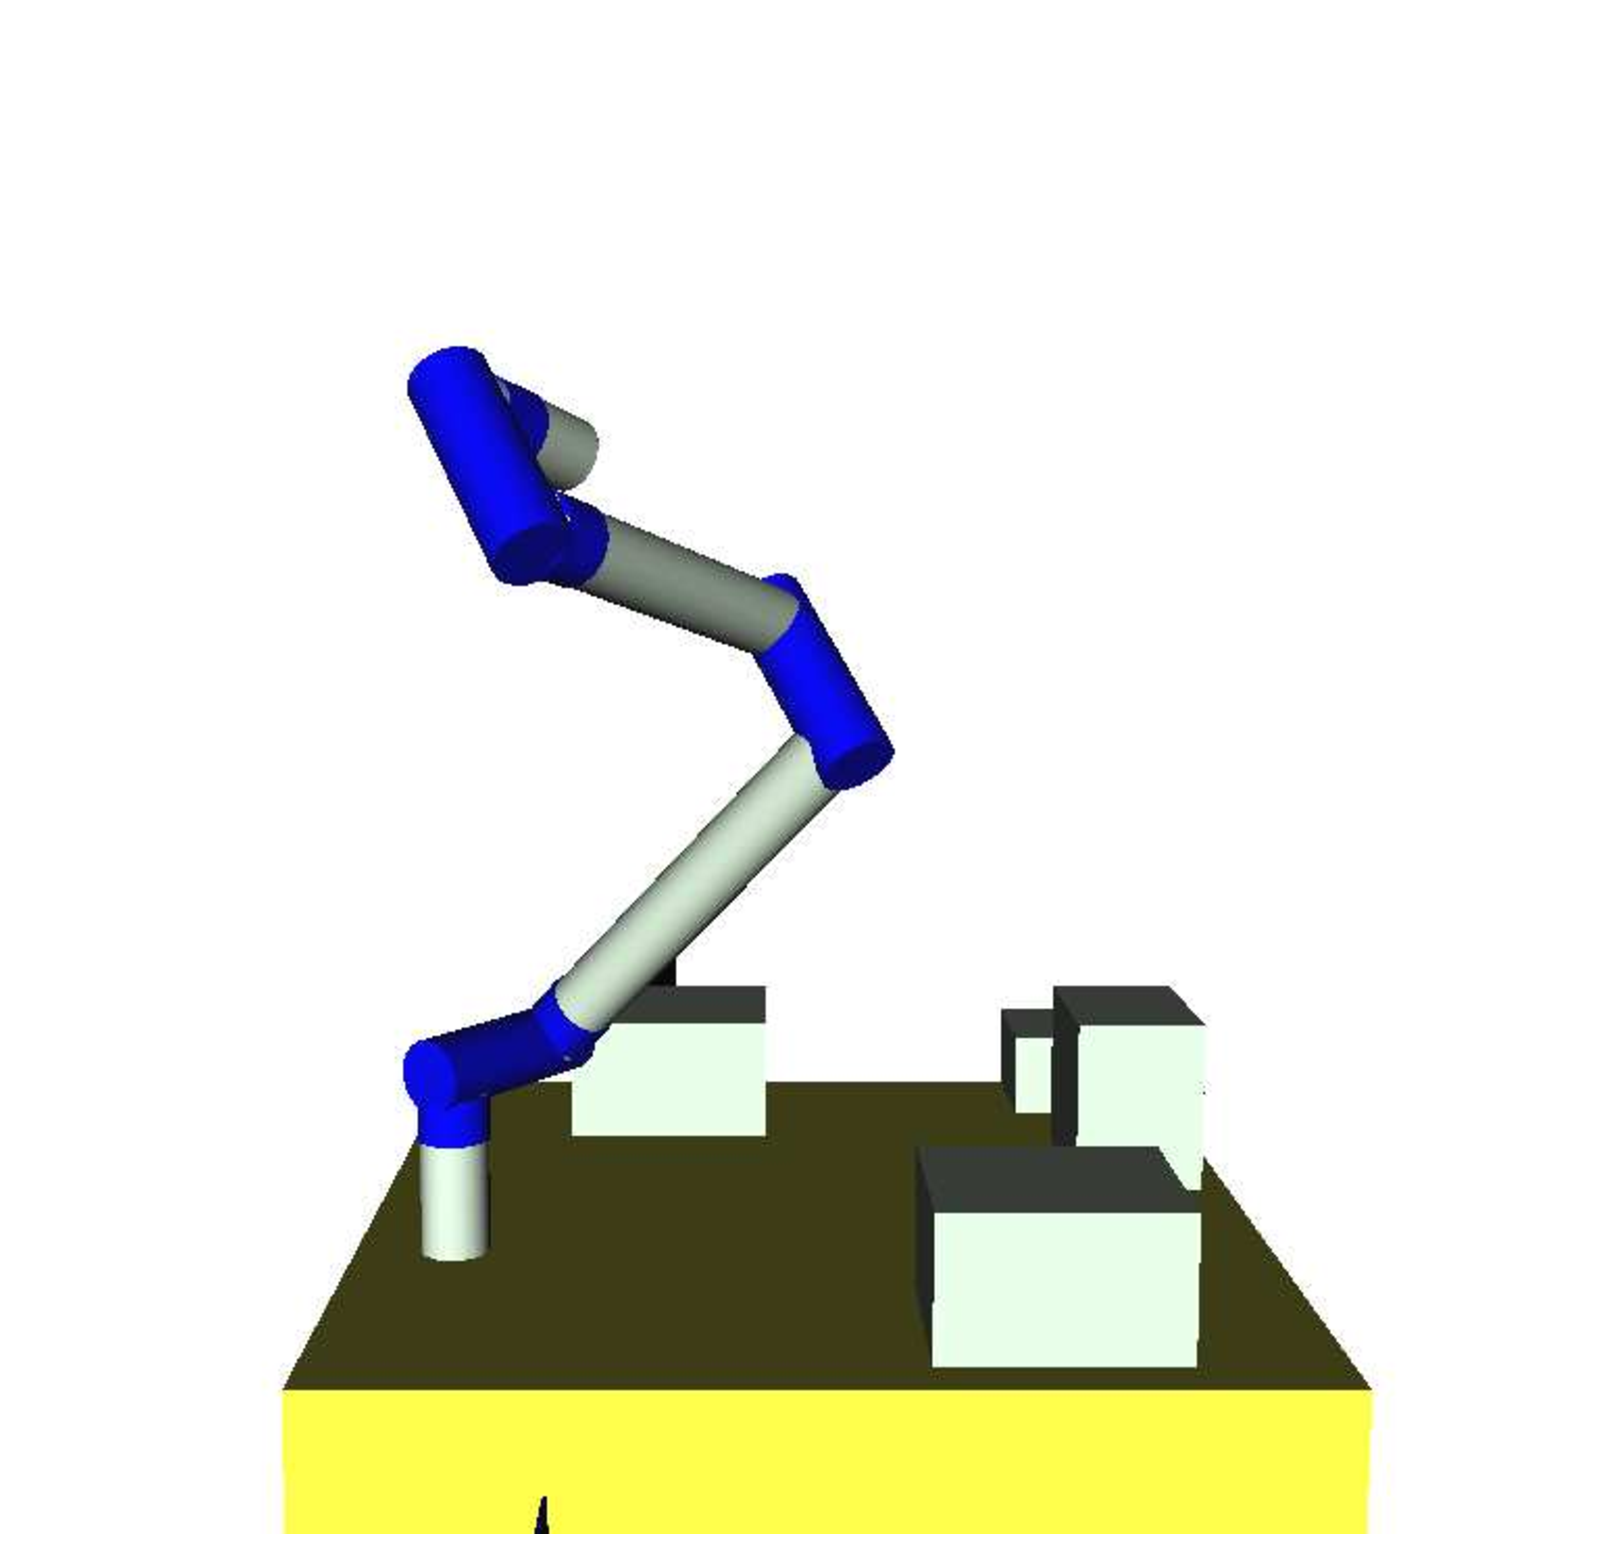
\includegraphics[width=1.0\linewidth]{fig/chapter4/deployment/03.eps}
    \centering
    \par\footnotesize{$t = 12.0~\mathrm{s}$}
  \end{minipage}\\
  \vspace{1em}
  \begin{minipage}[h]{0.28\linewidth}
    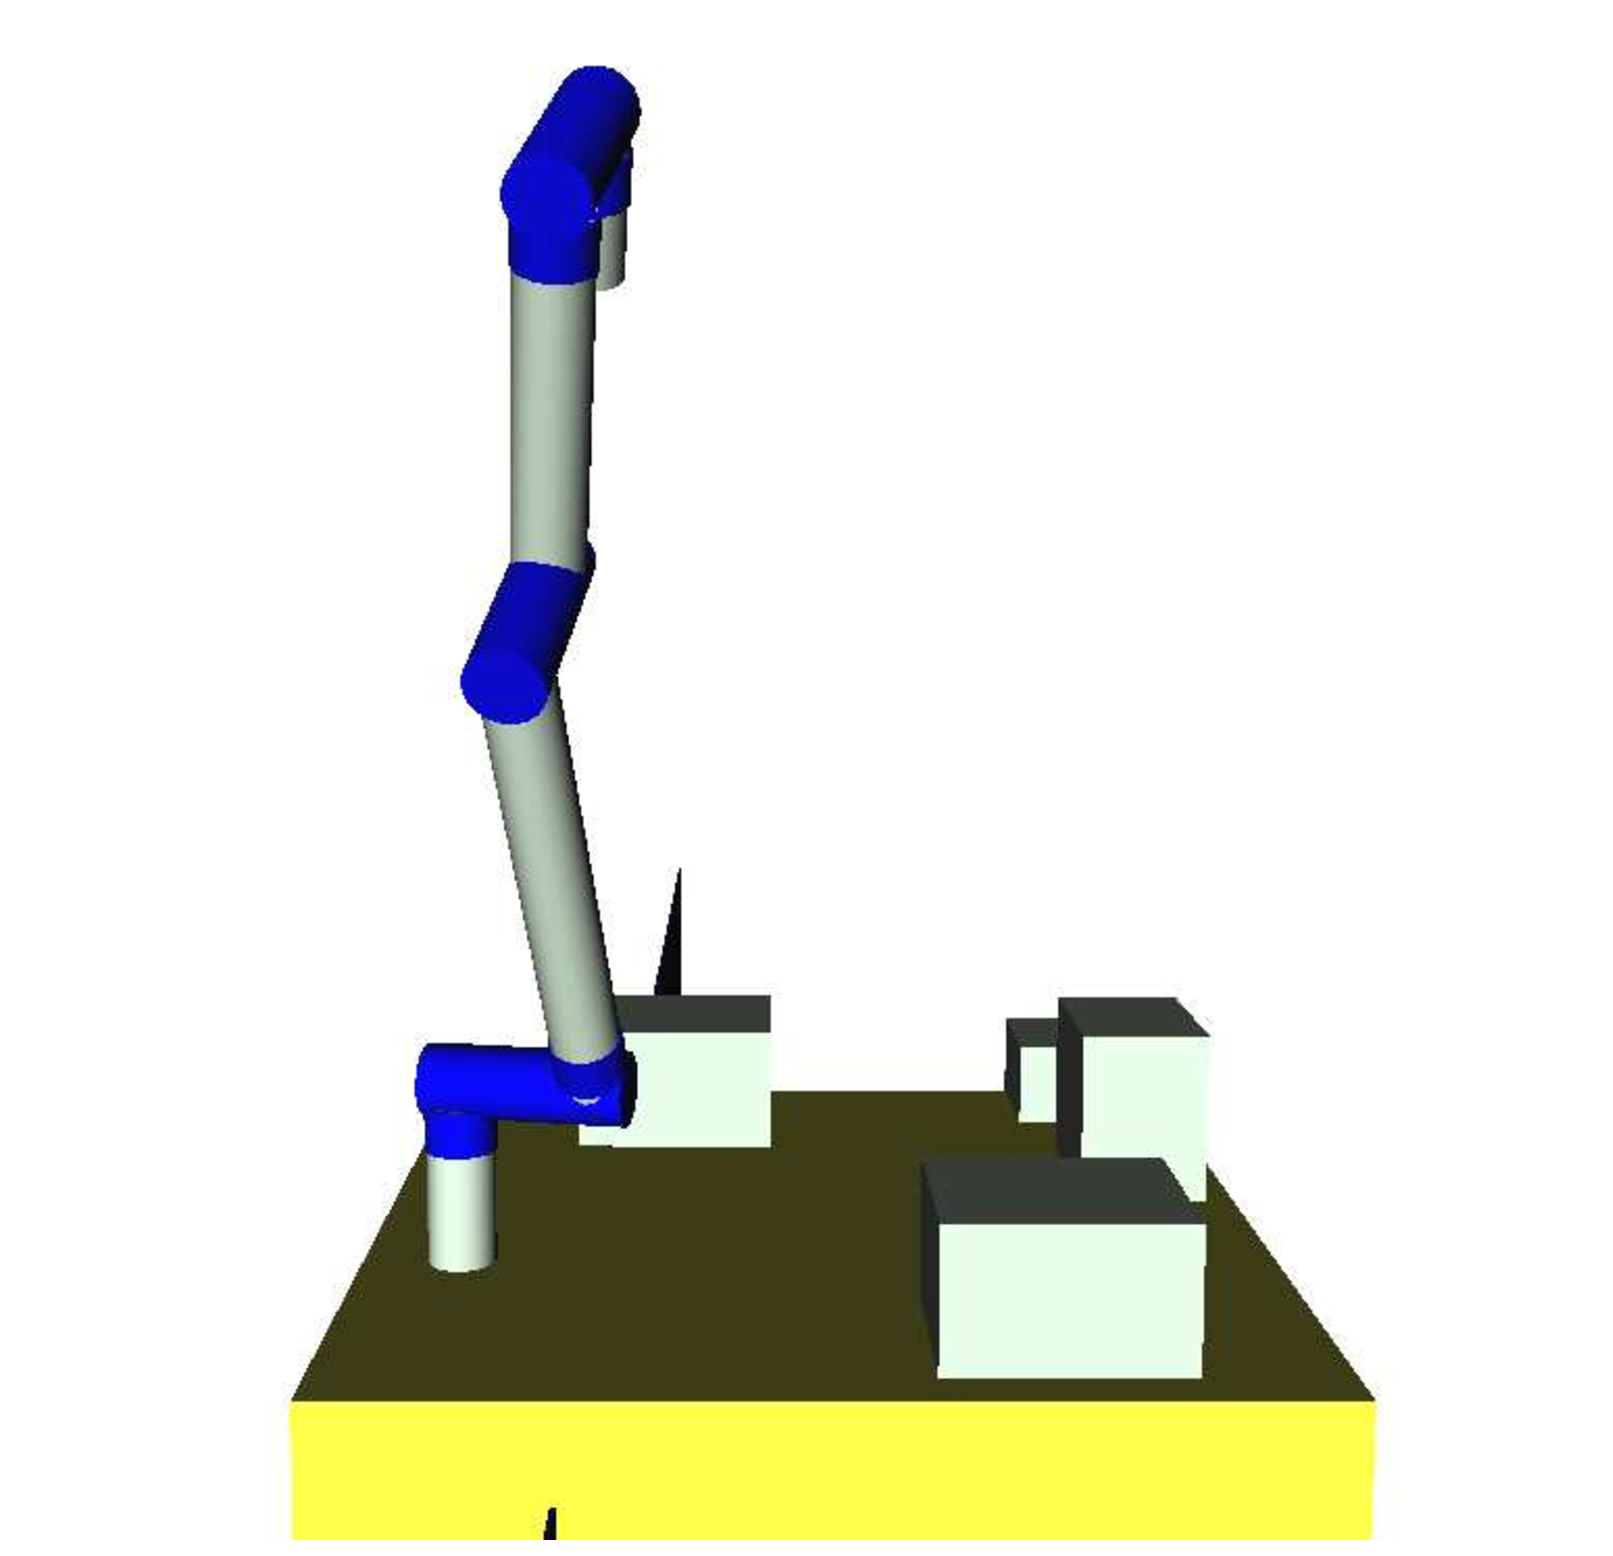
\includegraphics[width=1.0\linewidth]{fig/chapter4/deployment/04.eps}
    \centering
    \par\footnotesize{$t = 17.0~\mathrm{s}$}
  \end{minipage}
  \begin{minipage}[h]{0.28\linewidth}
    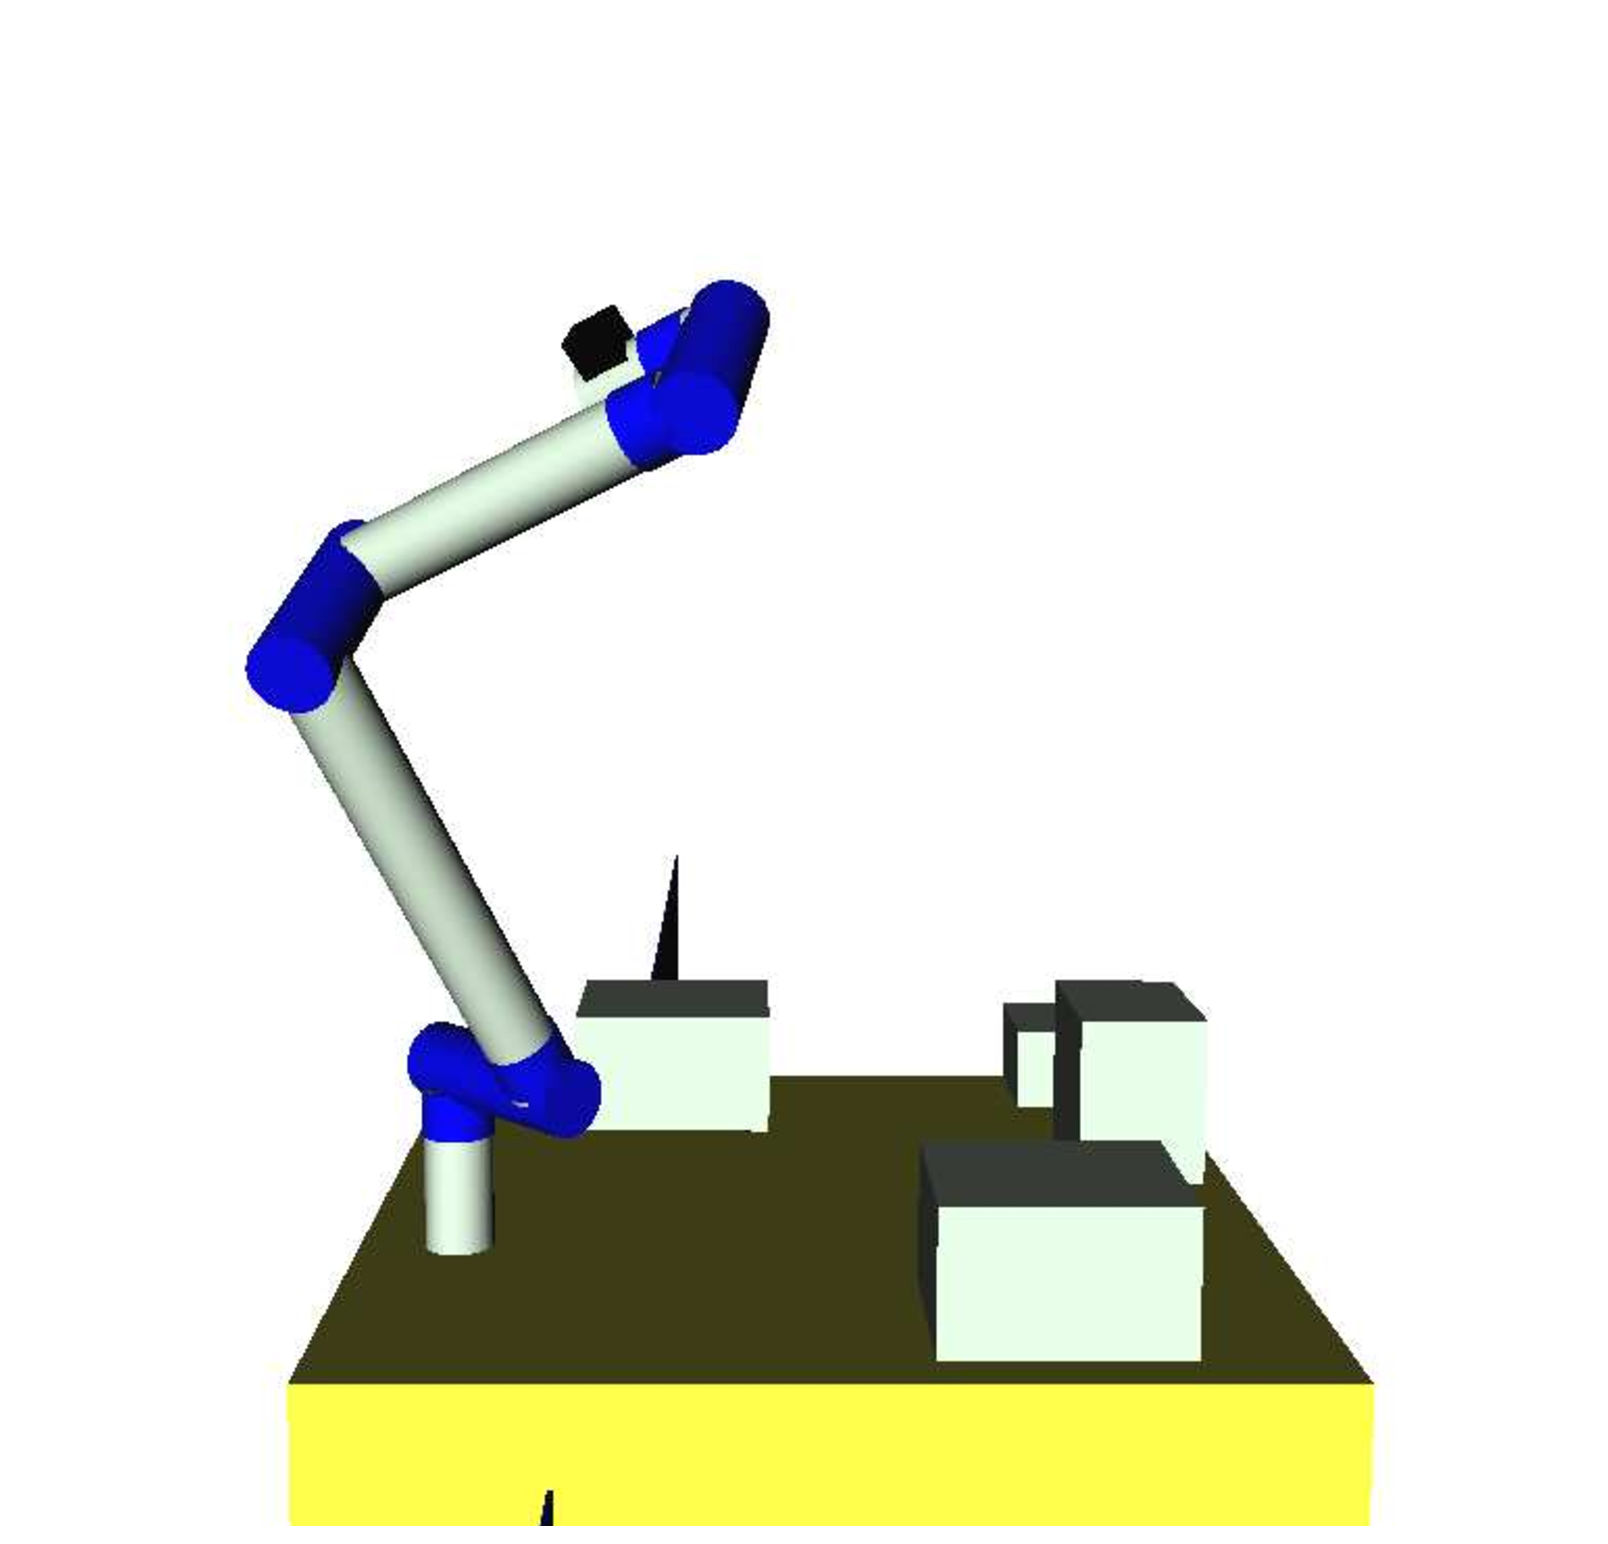
\includegraphics[width=1.0\linewidth]{fig/chapter4/deployment/05.eps}
    \centering
    \par\footnotesize{$t = 22.0~\mathrm{s}$}
  \end{minipage}
  \begin{minipage}[h]{0.28\linewidth}
      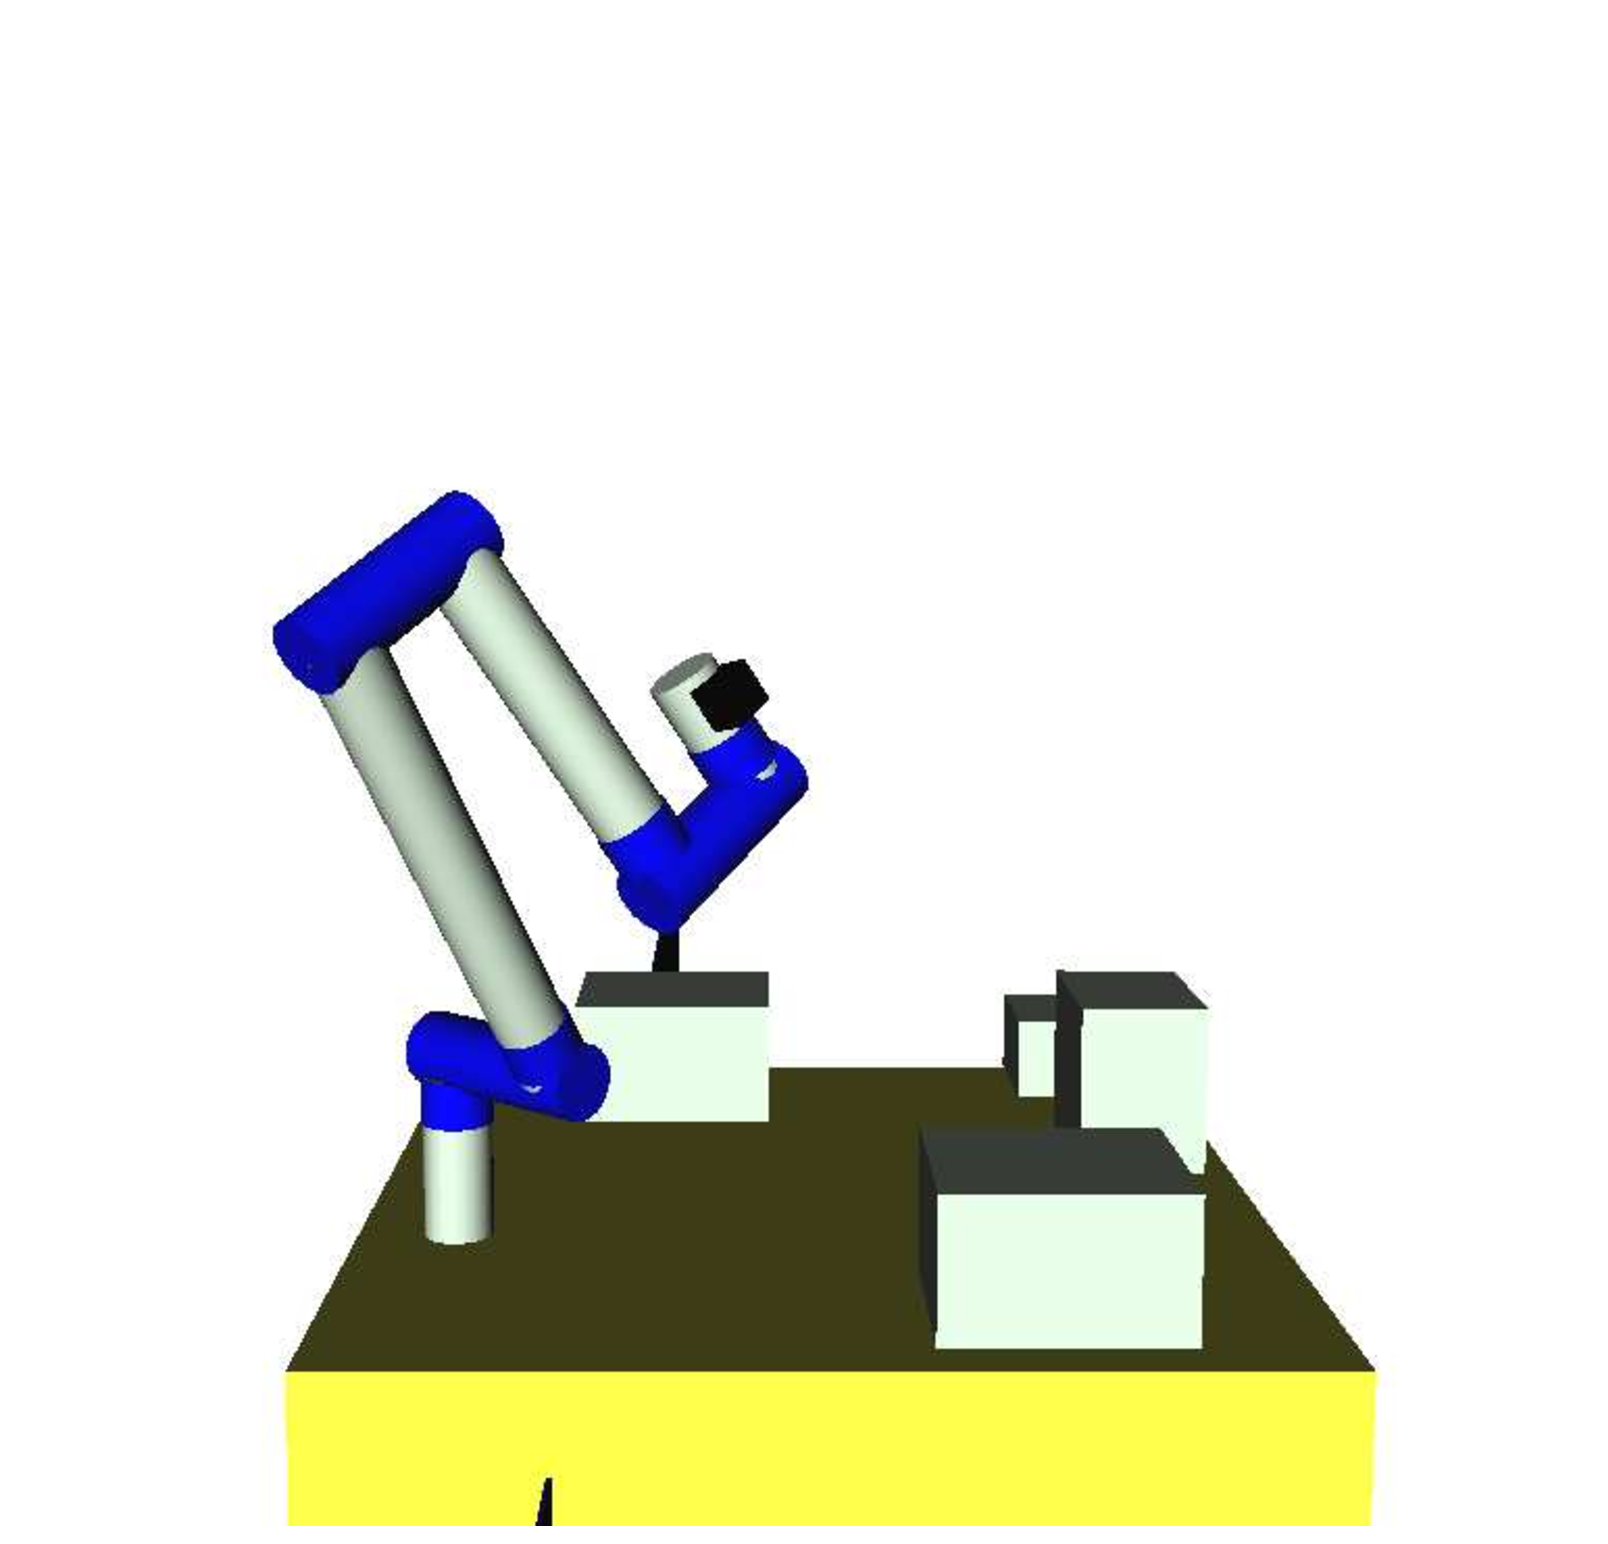
\includegraphics[width=1.0\linewidth]{fig/chapter4/deployment/06.eps}
      \centering
      \par\footnotesize{$t = 30.0~\mathrm{s}$}
    \end{minipage}
  \caption{Motion snapshots from the deployment task under reactionless motion control.}
  \label{fig:SNAP_DEPLOY}
\end{figure}
% ---------------------------------------------------------------------
%
It can be seen that the reactionless path is
passing through an appropriate point for an inspection task at $t = 30\unit{s}$.
In that case,
this motion task can be useful.
The possibility of the reactionless deployment was confirmed at least this case.

However, it should be noted that this motion task is only available when
a useful reactionless motion path can be prepared for specific tasks.
Instead of the full-reactionless motion,
we propose a deployment method using reactionless motion partially based on
the 3-phase method in what follows.

%%%%%%%%%%%%%%%%%%%%%%%%%%%%%%%%%%%%%%%%%%%%%%%
\subsubsection{Partial reactionless deployment}
%%%%%%%%%%%%%%%%%%%%%%%%%%%%%%%%%%%%%%%%%%%%%%%
Here, we present a deployment motion task for reduction of the base reaction.
We use a specific part of the 3-phase method;
in particular Phase II and III.
Because the stowed configuration is a folded configuration,
the sub-part of the 3-phase method can be used, straightforwardly.
From the results of the 3-phase method,
the base reaction can be reduced.

We show an example of the motion task.
The pre-positioning task for an inspection task, which was shown in \fig{ins}~(b), is assumed.
The initial configuration is set to the same stowed configuration that was used before.
The final configuration is set to $[90~50~0~-300~0~20~0]^{T}\unit{deg}$.
The middle point configuration at which the two motions are switched is obtained
as the terminal configuration from the final one
to the elbow folded configuration $\theta_{4} = \pi\unit{rad}$.

The snapshot of the motion task is displayed in \fig{SNAP_DEPLOY_PART}.
For comparison, the joint space controller with straight line trajectory was performed
under the same condition.
The snapshot is displayed in \fig{SNAP_DEPLOY_CONP}.
% \fig{RES_DEPLOY_PART} shows the time profile of the joint velocity,
% the base attitude on the both methods.
From the results, the maximum base attitude deviation under partial reactionless task was
$5.48\unit{deg}$;
on the other hand,
$7.66\unit{deg}$ base attitude was observed under the comparison controller.
Hence, $28.5\%$ reduction of the base attitude deviation can be realized.

%
% ---------------------------------------------------------------------
\begin{figure}[t]
  \centering
  \begin{minipage}[h]{0.32\linewidth}
    \includegraphics[width=1.0\linewidth]{fig/chapter4/deployment/partial/rls/01.eps}
      \centering
  \end{minipage}
  \begin{minipage}[h]{0.32\linewidth}
    \includegraphics[width=1.0\linewidth]{fig/chapter4/deployment/partial/rls/02.eps}
    \centering
  \end{minipage}
  \begin{minipage}[h]{0.32\linewidth}
    \includegraphics[width=1.0\linewidth]{fig/chapter4/deployment/partial/rls/03.eps}
    \centering
  \end{minipage}\\
  \vspace{1em}
  \begin{minipage}[h]{0.32\linewidth}
    \includegraphics[width=1.0\linewidth]{fig/chapter4/deployment/partial/rls/04.eps}
    \centering
  \end{minipage}
  \begin{minipage}[h]{0.32\linewidth}
    \includegraphics[width=1.0\linewidth]{fig/chapter4/deployment/partial/rls/05.eps}
    \centering
  \end{minipage}
  \begin{minipage}[h]{0.32\linewidth}
      \includegraphics[width=1.0\linewidth]{fig/chapter4/deployment/partial/rls/06.eps}
      \centering
    \end{minipage}
  \caption{The snapshot of the motion under partial reactionless deployment.}
  \label{fig:SNAP_DEPLOY_PART}
\end{figure}
% ---------------------------------------------------------------------
%
%
% ---------------------------------------------------------------------
\begin{figure}[t]
  \centering
  \begin{minipage}[h]{0.32\linewidth}
    \includegraphics[width=1.0\linewidth]{fig/chapter4/deployment/partial/conv/01.eps}
      \centering
  \end{minipage}
  \begin{minipage}[h]{0.32\linewidth}
    \includegraphics[width=1.0\linewidth]{fig/chapter4/deployment/partial/conv/02.eps}
    \centering
  \end{minipage}
  \begin{minipage}[h]{0.32\linewidth}
    \includegraphics[width=1.0\linewidth]{fig/chapter4/deployment/partial/conv/03.eps}
    \centering
  \end{minipage}\\
  \vspace{1em}
  \begin{minipage}[h]{0.32\linewidth}
    \includegraphics[width=1.0\linewidth]{fig/chapter4/deployment/partial/conv/04.eps}
    \centering
  \end{minipage}
  \begin{minipage}[h]{0.32\linewidth}
    \includegraphics[width=1.0\linewidth]{fig/chapter4/deployment/partial/conv/05.eps}
    \centering
  \end{minipage}
  \begin{minipage}[h]{0.32\linewidth}
      \includegraphics[width=1.0\linewidth]{fig/chapter4/deployment/partial/conv/06.eps}
      \centering
    \end{minipage}
  \caption{The snapshot of the motion under the conventional joint space interpolation.}
  \label{fig:SNAP_DEPLOY_CONP}
\end{figure}
% ---------------------------------------------------------------------
%


%%%%%%%%%%%%%%%%%%%%%
\section{Summary}
%%%%%%%%%%%%%%%%%%%%%
In this chapter,
we discussed the motion tasks that are suitable
for execution under reactionless motion control.
The following three tasks were considered:
(i) inspection task using a hand-held camera,
(ii) PTP positioning task and
(iii) deployment task from the stowed configuration.
We showed that the proposed methods using reactionless motion control
has a advantages compared with several conventional controllers in terms of
the base reaction.
% In addition, at the inspection task,
% we dealt with the algorithmic singularity stemming from the coupling between
% end-effector orientation control and the reactionless constraint.
% We showed that the singularity consistent method can alleviate the problem.











%**********************************************************************
%
%
%%% Local Variables:
%%% mode: latex
%%% TeX-master: "./main"
%%% End: